\documentclass[a4paper,12pt]{article}
\usepackage[utf8]{inputenc}
\usepackage{graphicx}
\usepackage{amsmath}
\usepackage[serbian]{babel}
\usepackage{url}
\usepackage[T1]{fontenc}
\usepackage{lmodern}
\renewcommand{\figurename}{Slika}  % Change "Figure" to "Slika"
\renewcommand{\tablename}{Tabela}
\begin{document}

\begin{titlepage}
    \centering
	\begin{figure}[htbp]
    	\centering
    	
\includegraphics[width=0.4\textwidth]{./images/logo.png}
	\end{figure}
    { Univerzitet u Beogradu \\ Matematički fakultet\par}
	
    \vfill

    {\Large \textbf{Seminarski rad}\par}

    \vspace{1cm}

    {\Large \textbf{Analiza, klasifikacija i klasterovanje proteinskih blokova}\par}

    \vfill

    
	
	
	\begin{tabbing}
	\hspace{10cm} \= \hspace{10cm} \= \kill
	\textbf{Mentor:} \>  \textbf{Studenti:} \\
	Prof. dr Nenad Mitić \> Anja Milutinović 235/2021 \\
	Katedra za računarstvo i informatiku \> Đurđa Milošević 84/2021 \\
	\> Smer: Informatika
	\end{tabbing}

    \vfill

    \textbf{Datum:} 2024/25

\end{titlepage}
\newpage
\tableofcontents
\newpage
\section{Uvod}
Proteini su osnovni gradivni blokovi svih ćelija u organizmu i kao takvi igraju ključnu ulogu u održavanju života, reprodukciji, odbrani i replikaciji. Funkcije proteina zavise od njihove strukture, zbog čega je analiza strukture proteina od izuzetnog značaja u bioinformatičkim i biohemijskim istraživanjima.\\
\\
U nastojanju da se postigne precizniji, detaljniji i informativniji prikaz trodimenzionalne strukture proteina, razvijeni su proteinski blokovi. Kao jedni od najistaknutijih predstavnika strukturnih alfabeta, pokazano je da omogućavaju detekciju strukturne sličnosti između proteina sa izuzetnom efikasnošću.\\
\\
Ovaj seminarski rad se fokusira na proteinske blokove, sa posebnim akcentom na retke i neočekivane prelaze između njih. Niz proteinskih blokova dobijen je analizom humanog proteoma, koji je generisan pomoću AlphaFold2 programa. Seminarski rad se sastoji od tri ključna segmenta: analize, klasifikacije i klasterovanja proteinskih blokova.\\
Analiza obuhvata izdvajanje aminokiselina i sekundarnih struktura u retkim prelazima, određivanje prirode vrednosti pLDDT (eng. \textit{the predicted local distance difference test}) i RSA (eng. \textit{relative solvent accessibility}) parametara, kao i poređenje zastupljenosti pojedinačnih aminokiselina u podacima u odnosu na očekivane procente. \\
Klasifikacija je usredsređena na predviđanje aminokiselina i sekundarnih struktura u prelazima, kao i parova proteinskih blokova koji čine posmatrane prelaze. Ovaj pristup omogućava donošenje interesantnih zaključaka o relevantnosti, ubedljivosti i stabilnosti proteinskih blokova kao strukturnih indikatora. \\
Klasterovanje je izvedeno nad skupom podataka koji sadrži informacije o strukturi proteina, uključujući prelaze između proteinskih blokova, kao i aminokiseline i sekundarne strukture prisutne u tim prelazima. \\
\\
Seminarski rad je realizovan u okviru kursa „Istraživanje podataka 2” na Matematičkom fakultetu Univerziteta u Beogradu.
\newpage
\section{O Proteinskim blokovima}
Pronalaženje sličnosti u prostornoj strukturi proteina je važno jer može da ukaže na sličnosti u funkcionalnosti proteina, koja nije vidljiva ispitivanjem sekvencijalnih informacija o proteinu. Eksperimentalno određivanje trodimenionalne strukture proteina je skup i vremenski zahtevan proces. Zato, potrebno je da se pronađe efikasan i pouzdan način opisivanja trodimenzionalne strukture proteina, kao i način upoređivanje više struktura proteina međusobno.
\\
Struktura proteina se obično opisuje kao $\alpha$-heliks ili $\beta$-ravan. zasnovano na vodoničnim vezama između peptidnih veza unutar glavnog lanca proteina, ali ovaj pristup se pokazao previše uprošćen jer preko 50\% strukture proteina ostaje neopisano.\cite{debrevern2010proteinblocks}
Trodimenzionalna struktura može se opisati i korišćennjem aproksimativnih prototipova lokalne strukture proteina. Skup definisanih prototipova lokalne strukture se naziva i strukturni alfabet. Direktno određivanje trodimenizionalne strukture proteina je težak problem, zato se koriste strukturni alfabeti koji opisuju trodimenzionalnu strukturu proteina jednodimenzionalnim nizom strukturnih prototipova. 

\begin{figure}[h!]
    \centering
    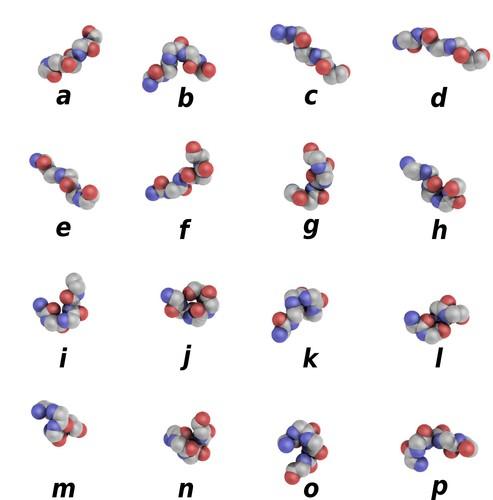
\includegraphics[width=0.7\textwidth]{./images/PBs.jpg}
    \caption{Šematski prikaz 16 proteinskih blokova označenh slovima od a do p}
    \label{Slika:pbs}
\end{figure}

Jedan od najpoznatijih strukturnih alfabeta jeste Proteinski blokovi (PB), koje je razvio De Brevern. Proteinski blokovi se sastoji od 16 prototipova, koji su izdvojeni korišćenjem algoritama klasterovanja, Kohenonove samoorganizovajuće mape, nad fragmentima od pet uzastopnih aminokiselina kod proteina sa već poznatom strukturom. U prvom istraživanju je korišćeno 228 poznatih proteina, a kasnije je istraživanje ponovljeno nad 400 poznatih proteina. Procedura klasterovanja se odvijala u tri koraka. U prvom koraku se koristi mera sličnosti fragmenata RMSDA (eng. Root Mean Square Deviation on Angle), u drugom koraku se dodatno koristi i verovatnoća prelaska jednog fragmenta u drugi u sekvenci, dok se u trećem koraku izbacuje ograničenje verovatnoće prelaska. Na kraju je odabrano 16 proteinskih blokova, definisanih sa osam diedarskih uglova, $\psi_{i-2}$, $\phi_{i-1}$, $\psi_{i-1}$, $\phi_i$, $\psi_i$, $\phi_{i+1}$, $\psi_{i+1}$, $\phi_{i+2}$ u odnosu na centralnu aminokiselinu u fragmentu dužine pet. \cite{joseph2010biohysrev} (Tabela \ref{Tabela:1})
\\
\begin{table}[h!]
    \centering
    \begin{tabular}{|c|c|c|c|c|c|c|c|c|}
        \hline
        \textbf{PB} & \textbf{$\psi_{i-2}$} & \textbf{$\phi_{i-1}$} & \textbf{$\psi_{i-1}$} & \textbf{$\phi_i$} & \textbf{$\psi_i$} & \textbf{$\phi_{i+1}$} & \textbf{$\psi_{i+1}$} & \textbf{$\phi_{i+2}$ } \\
        \hline
        a & 41.14 & 75.53 & 13.92 & -99.80 & 131.88 & -96.27 & 122.08 & -99.68 \\ \hline
        b & 108.24 & -90.12 & 119.54 & -92.21 & -18.06 & -128.93 & 147.04 & -99.90 \\ \hline
        c & -11.61 & -105.66 & 94.81 & -106.09 & 133.56 & -106.93 & 135.97 & -100.63 \\ \hline
        d & 141.98 & -112.79 & 132.20 & -114.79 & 140.11 & -111.05 & 139.54 & -103.16 \\ \hline
        e & 133.25 & -112.37 & 137.64 & -108.13 & 133.00 & -87.30 & 120.54 & 77.40 \\ \hline
        f & 116.40 & -105.53 & 129.32 & -96.68 & 140.72 & -74.19 & -26.65 & -94.51 \\ \hline
        g & 0.40   & -81.83 & 4.91 & -100.59 & 85.50 & -71.65 & 130.78 & 84.98 \\ \hline
        h & 119.14 & -102.58 & 130.83 & -67.91 & 121.55 & 76.25 & -2.95 & -99.88 \\ \hline
        i & 130.68 & -56.92 & 119.26 & 77.85 & 10.42 & -99.43 & 141.40 & -98.01 \\ \hline
        j & 114.32 & -121.47 & 118.14 & 82.88 & -150.05 & -83.81 & 23.35 & -85.82 \\ \hline
        k & 117.16 & -95.41 & 140.40 & -59.35 & -29.23 & -72.39 & -25.08 & -76.16 \\ \hline
        l & 139.20 & -55.96 & -32.70 & -68.51 & -26.09 & -74.44 & -22.60 & -71.74 \\ \hline
        m & -39.62 & -64.73 & -39.52 & -65.54 & -38.88 & -66.89 & -37.76 & -70.19 \\ \hline
        n & -35.34 & -65.03 & -38.12 & -66.34 & -29.51 & -89.10 & -2.91 & 77.90 \\ \hline
        o & -45.29 & -67.44 & -27.72 & -87.27 & 5.13 & 77.49 & 30.71 & -93.23 \\ \hline
        p & -27.09 & -86.14 & 0.30 & 59.85 & 21.51 & -96.30 & 132.67 & -92.91 \\ \hline
    \end{tabular}
	\caption{Referentni uglovi Proteinskih blokova}
	\label{Tabela:1}
\end{table}
\newpage
Proteinski blokovi su označeni slovima od a do p (Slika \ref{Slika:pbs}). Najčešći proteinski blokovi, m i d, odgovaraju redom alfa-heliksu i beta-ravni. Proteinski blokovi od g do j odgovaraju nespecificnim strukturama (eng. coil). \\
Prevođenje u sekvencu proteinskih blokova kod proteina sa poznatom 3D strukturom odvija se tako što se svakom fragmentu uzastopnih aminokselina dužine pet dodeli jedan proteinski blok sa najmanjom vrednošću RMSDA-a. U slučajevima kada izračunavanje diedralnih uglova nije moguće, kao i na krajevima lanca gde se ne može formirati prozor od pet aminokiselina, dodeljuje se slovo Z. Na ovaj način svaka aminokiselina učestvuje u pet proteinskih blokova, osim prve i poslednje. \\
Strukturni alfabet Proteinski blokovi se koristi i u drugim podoblastima bioinformatike kao što su nadređivanje 3D strukture proteina, istraživanje strukture proteina, definisanje mesta vezivanja, i analize lokalnih konformacija poremećenih proteina. \\
Postoje alati koji prevode PDB datoteke u sekvence proteinskih blokova, kao što je PBxplore.
\newpage
\section{Analiza}
U ovom poglavlju analizirani su prelazi između proteinskih blokova. Fokus analize bio je na identifikaciji neočekivanih prelaza između proteinskih blokova i proučavanju aminokiselina i sekundarnih struktura prisutnih u njima. Analiza koja se odnosi na aminokiseline i sekundarne strukture sprovedena je nad skupom podataka \texttt{March\_2024\_PDB\_01.txt}, dok su ispitivanje vrednosti relevantnih parametara (\texttt{pLDDT} i \texttt{RSA}) i analiza zastupljenosti pojedinačnih aminokiselina u podacima izvršeni na osnovu datoteke \texttt{March\_2024\_AF2\_01.txt}.

\subsection{Opis podataka}
Podaci korišćeni u analizi obuhvataju informacije o proteinskim blokovima (PBs), aminokiselinama (AA), sekundarnim strukturama (S2), predviđenoj učestalosti prelaza, kao i dodatnim parametrima poput pLDDT i RSA. Izvor podataka su rezultati generisani pomoću AlphaFold2 programa. Konkretno, analiza je sprovedena nad dve datoteke: prvobitnog, obimnijeg skupa podataka, koji detaljnije opisuje prelaze između proteinskih blokova i manjeg podskupa dobijenog filtriranjem rezultata u skladu sa humanim proteomom. \\
Podaci su organizovani u tabelarnom formatu, pri čemu svaki red sadrži parove proteinskih blokova koji čine prelaz, parove aminokiselina i sekundarnih struktura koji ga opisuju, predviđenu učestalost prelaza i vrednosti parametara pLDDT i RSA.
\\
U nastavku je prikazan opis atributa datoteke \texttt{March\_2024\_AF2\_01.txt}.  
Datoteka \texttt{March\_2024\_PDB\_01.txt} sadrži identičan skup atributa, izuzev atributa \texttt{pLDDT} i \texttt{RSA}:

\begin{itemize}
    \item \textbf{Protein\_number} – diskretan, kategorijski i redni atribut koji označava pojedinačne proteine u skupu podataka.
    \item \textbf{res\_number} – diskretan, kategorijski i redni atribut koji označava poziciju aminokiselinskog ostatka unutar sekvence.
    \item \textbf{PB1, PB2} – diskretni, kategorijski i nominalni atributi koji predstavljaju oznake proteinskih blokova između kojih dolazi do prelaza.
    \item \textbf{AA1, AA2} – diskretni, kategorijski i nominalni atributi koji opisuju aminokiseline prisutne u prelazu. Postoji ukupno 20 različitih vrednosti za ove atribute, u skladu sa standardnim skupom aminokiselina koje grade proteine. U tabeli \ref{Tabela:2} prikazane su odgovarajuće jednoslovne oznake za svaku aminokiselinu.
\begin{table}[h!]
    \centering
	\begin{tabular}{ |l|c| } 
	\hline
	\textbf{Aminokiselina} &  \textbf{Jednoslovna oznaka}\\
	\hline
	Alanin &	 A \\
	\hline
	Arginin 	& R 	\\
	\hline
	Asparagin &	N \\
	\hline
	Asparaginska kiselina & D \\
	\hline
	Cistein 	& C 	\\
	\hline
	Glutaminska kiselina & E \\
	\hline
	Glutamin & Q \\
	\hline
	Glicin & G \\
	\hline
	Histidin & H \\
	\hline
	Izoleucin & I \\
	\hline
	Leucin & L \\
	\hline
	Lizin &	K \\
	\hline
	Metionin & M \\
	\hline
	Fenilalanin & F \\
	\hline
	Prolin & P \\
	\hline
	Serin & S \\
	\hline
	Treonin 	& T \\
	\hline
	Triptofan & W \\
	\hline
	Tirozin 	& Y \\
	\hline
	Valin & V  \\
	\hline
	\end{tabular}
	\caption{Aminokiseline i njihove jednoslovne oznake korišćene kao vrednosti atributa AA1 i AA2.}
	\label{Tabela:2}
\end{table}
\newpage
    \item \textbf{S2\_1, S2\_2} – diskretni, kategorijski i nominalni atributi koji predstavljaju sekundarne strukture prisutne u prelazu. Vrednosti ovih atributa određene su pomoću DSSP (\textit{eng. Dictionary of Secondary Structure of Proteins}) programa~\cite{carter2003dsspcont}. DSSP program se koristi za dodeljivanje jednog od osam stanja sekundarne strukture aminokiselinama tako što se identifikuju vodonične veze između amino i karboksilnih grupa glavnog lanca proteina. \\
U tabeli \ref{Tabela:3} prikazane su oznake i odgovarajući tipovi sekundarne strukture.
\\
\begin{table}[h!]
    \centering
    \begin{tabular}{ |c|l| } 
    \hline
    \textbf{Oznaka} & \textbf{Tip sekundarne strukture} \\
    \hline
    H & Alfa-heliks (\textit{eng. $\alpha$-helix}) \\
    B & Beta-most (\textit{eng. beta bridge}) \\
    E & Prošireni beta list (\textit{eng. extended beta sheet}) \\
    G & 3(10)-heliks \\
    I & Pi-heliks (\textit{eng. $\pi$-helix}) \\
    T & Heliks okret (\textit{eng. helix-turn}) \\
    S & Zavojnica (\textit{eng. bend}) \\
    C & Nespecifična ili neorganizovana struktura (\textit{eng. coil}) \\
    \hline
    \end{tabular}
    \caption{Sekundarne strukture proteina prema DSSP programu, korišćene kao vrednosti atributa S2\_1 i S2\_2.}
    \label{Tabela:3}
\end{table}
\newpage
    \item \textbf{expected\_frequency} - neprekidan, kvantitativan i razmerni atribut čija vrednost pripada intervalu [0,1] i označava očekivanu učestalost prelaza između proteinskih blokova.
    \item \textbf{pLDDT, RSA1, RSA2} – neprekidni, kvantitativni i razmerni atributi čije su vrednosti u intervalu [0,100]. Parametar pLDDT procenjuje pouzdanost predikcije lokalne strukture proteina, dok RSA1 i RSA2 predstavljaju relativnu izloženost aminokiselinskih ostataka rastvaraču.
\end{itemize}
\subsection{Izdvajanje retkih prelaza između proteinskih blokova u podacima}
Glavni zadatak analize bio je proučavanje prelaza između proteinskih blokova, pri čemu je akcenat stavljen na neočekivane, retke prelaze. Takvi prelazi su, zbog svoje prirode, od posebnog interesa za istraživanje jer mogu doprineti novim saznanjima o nizu proteinskih blokova koji opisuje trodimenzionalnu strukturu proteina.  

U okviru implementacije, za potrebe filtriranja konstruisana je pomoćna funkcija \texttt{filter\_data\_set}, čiji je zadatak bio da ukloni kolone koje nisu od značaja za analizu, a zatim formira novu kolonu koja predstavlja spoj proteinskih blokova između kojih se prelaz ispituje. Nakon toga računaju se učestalosti svakog prelaza i generiše se tabela sa njihovim apsolutnim brojevima pojavljivanja. Na ovaj način dobijena je lista svih mogućih prelaza između proteinskih blokova sa pripadajućim brojem ponavljanja u posmatranom skupu podataka.  

Polazeći od ovako pripremljenih rezultata, izvršeno je izdvajanje onih prelaza čija relativna učestalost iznosi manje od $1\%$ u odnosu na ukupan broj prelaza. Konkretno, prelaz je označen kao \emph{redak} ukoliko se javlja u manje od $1\%$ svih slučajeva. Nakon toga je sprovedeno uklanjanje duplikata, čime je obezbeđeno da se retki prelazi posmatraju kao jedinstvene kombinacije proteinskih blokova. Konačan rezultat postupka predstavlja skup neočekivanih prelaza između proteinskih blokova koji su predmet daljih analiza. \\
Svi izdvojeni retki prelazi sačuvani su u datoteci \texttt{unexpected\_transitions.csv}.

\subsection{Izdvajanje parova aminokiselina prisutnih u neočekivanim prelazima}
U cilju pronalaženja potencijalnih korelacija između atributa, odnosno između parova aminokiselina vezanih za retki prelaz i proteinskih blokova koji formiraju prelaz, izvršeno je izdvajanje tih parova. Pored toga, izračunate su frekvencije svih parova, a zatim su izdvojeni oni najfrekventiniji. \\ 
S obzirom na to da se u podacima korišćenim za ovu analizu prelazi ne nadovezuju, posmatran je pojedinačno svaki prelaz i unutar njega određen svaki par aminokiselina. Važno je napomenuti da redosled aminokiselina u paru nije irelevantan, zbog čega se parovi aminokiselina (A1, A2) ne mogu smatrati identičnim parovima (A2, A1). Kako bi ova tvrdnja bila intuitivnija i jasnija, potrebno je prvo objasniti zašto je prelaz određen sa dve aminokiseline iako su proteinski blokovi sačinjeni od 5 uzastopnih aminokiselina. \\ 
Naime, prilikom dodeljivanja proteinskog bloka fragmentu od 5 aminokiselina, centralna aminokiselina igra ključnu ulogu  jer je ona ta koja efektivno definiše fragment i omogućava izračunavanje 8 diedarskih uglova $\psi_{i-2}$, $\phi_{i-1}$, $\psi_{i-1}$, $\phi_i$, $\psi_i$, $\phi_{i+1}$, $\psi_{i+1}$, $\phi_{i+2}$.  Ovi uglovi se zatim upoređuju sa već definisanim diedarskim uglovima prototipova proteinskih blokova nakon čega se dodeljuje odgovarajući proteinski blok. Dakle, za svaki prelaz centralna aminokiselina je najvažnija zbog njenog uticaja na ceo fragment i zato je baš ona ta koja je izabrana da bude deo podataka, odnosno da bude predstavnik u prelazu. 

Imajući u vidu prethodno navedeno, obrnut redosled aminokiselina u paru može da predstavlja potpuno različit prelaz između proteinskih blokova i zato je važno analizirati ih kao zasebne parove. Slika \ref{Slika:aa} prikazuje primer iz skupa podataka koji ilustruje iznesenu tvrdnju.
\begin{figure}[htbp]
    \centering
    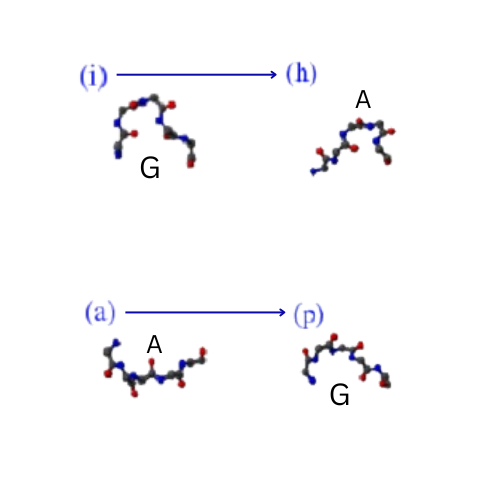
\includegraphics[width=0.5\textwidth]{./images/aa.png}
    \caption{Redosled aminokiselina u paru je važan.}
    \label{Slika:aa}
\end{figure}
\\
Izračunate su frekvencije svakog para aminokiselina u prelazima. Najčešće se javlja par (G, G). Pregled ostalih 19 najučestalijih parova dat je na slici \ref{Slika:aafreq}.
\begin{figure}[htbp]
    \centering
    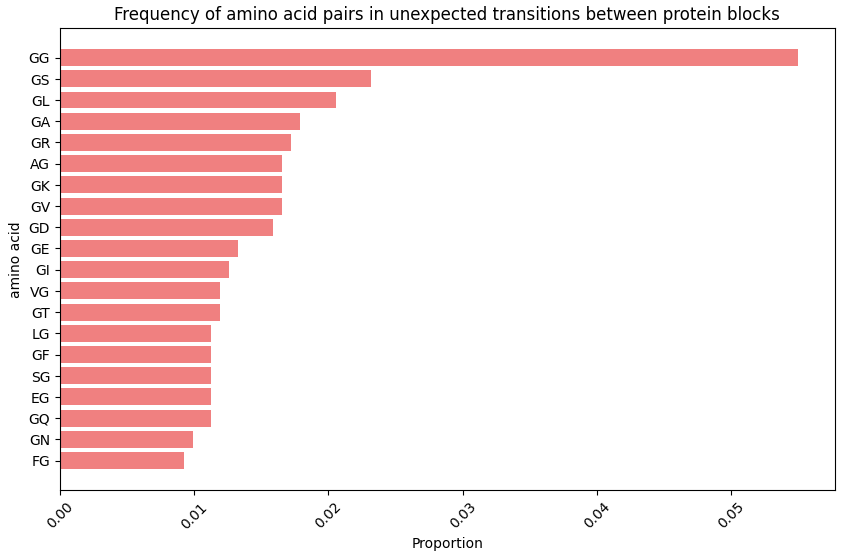
\includegraphics[width=1\textwidth]{./images/aafreq.png}
    \caption{Frekvencija parova aminokiselina u retkim prelazima.}
    \label{Slika:aafreq}
\end{figure}
\newpage
Dobijeni najfrekventniji par je od posebnog interesa s obzirom na specifične karakteristike glicina.
Glicin, zbog svog malog bočnog lanca, ima ključnu ulogu u omogućavanju fleksibilnosti u proteinu. Takođe, glicin doprinosi stabilnosti tercijalne strukture proteina \cite{dong2012glycines}. S obzirom na to, njegova velika učestalost može ukazivati na stabilnost u prelazima.\\
Svi parovi aminokiselina, zajedno sa njihovim frekvencijama, sačuvani su u datoteci \texttt{amino\_acid\_pairs.csv}.
\subsection{Izdvajanje parova sekundarnih struktura koji se javljaju u neočekivanim prelazima}
Nakon izdvajanja aminokiselina, sledeći korak u analizi bio je ispitivanje sekundarnih struktura koje se javljaju u prelazima i njihove učestalosti. Kao i u slučaju aminokiselina, izvojeni su parovi sekundarnih struktura tako da je redosled unutar svakog para važan. \\
Sekundarna struktura proteina definiše lokalne konformacije polipeptidnog lanca koje nastaju usled interakcija između atoma kičme lanca. Najčešča klasifikacija sekundarne strukture je na $\alpha$-zavojnice i $\beta$-ploče, dok se ostale konformacije označavaju kao neregularno stanje (\textit{eng. coil}). Međutim, utvrđeno je da u proseku čak $50\%$ ostataka \cite{debrevern2010proteinblocks} kolektivno tretira kao neregularno stanje što značajno pojednostavljuje strukturu proteina i dovodi do brojnih ograničenja u njenoj analizi. To je jedan od glavnih razloga formiranja proteinskih blokova kao koncepta. \\ 
U skladu sa tim, očekuje se da će analiza parova sekundarnih struktura u retkim prelazima između proteinskih blokova pokazati pretežnu zastupljenost neregularnih stanja, odnosno \textit{coil}, pošto sami proteinski blokovi treba što vernije da opišu upravo one konformacije koje se ne mogu jednostavno klasifikovati kao $\alpha$-zavojnice i $\beta$-ploče, niti njihove varijacije (E - \textit{extended beta sheet}, G - \textit{(10)-helix)}). \\
Izračunate su frekvencije parova sekundarnih struktura u prelazima i na slici \ref{Slika:s2freq} su prikazani oni najučestaliji, odnosno dvadeset najučestalijih parova.
\begin{figure}[htbp]
    \centering
    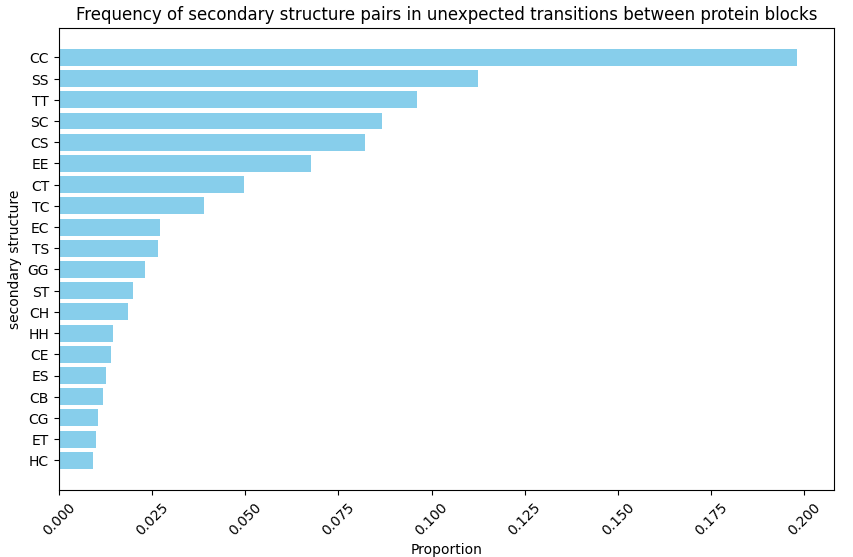
\includegraphics[width=1\textwidth]{./images/s2freq.png}
    \caption{Frekvencija parova sekundarnih struktura u retkim prelazima.}
    \label{Slika:s2freq}
\end{figure}
\\
Rezultati analize pokazuju da su najčešće zastupljeni parovi CC (\textit{coil–coil}), SS (\textit{bend–bend}) i TT (\textit{helix-turn–helix-turn}), koji ne pripadaju klasičnim tipovima sekundarnih struktura. Ovo je u skladu sa pretpostavkom da će u retkim prelazima dominirati neregularne sekundarne strukture. \\
Svi parovi sekundarnih struktura, zajedno sa njihovim frekvencijama, sačuvani su u datoteci \texttt{secondary\_structure\_pairs.csv}.
\subsubsection{Izdvajanje kombinacija aminokiselina i sekundarnih struktura u neočekivanim prelazima}
Pored analize parova aminokiselina i sekundarnih struktura zasebno, izvršeno je i ispitivanje njihovih kombinacija radi pronalaska međusobnih korelacija u prelazima.  \\
Na slici \ref{Slika:aas2freq} dat je prikaz najfrekventnijih kombinacija.
\begin{figure}[htbp]
    \centering
    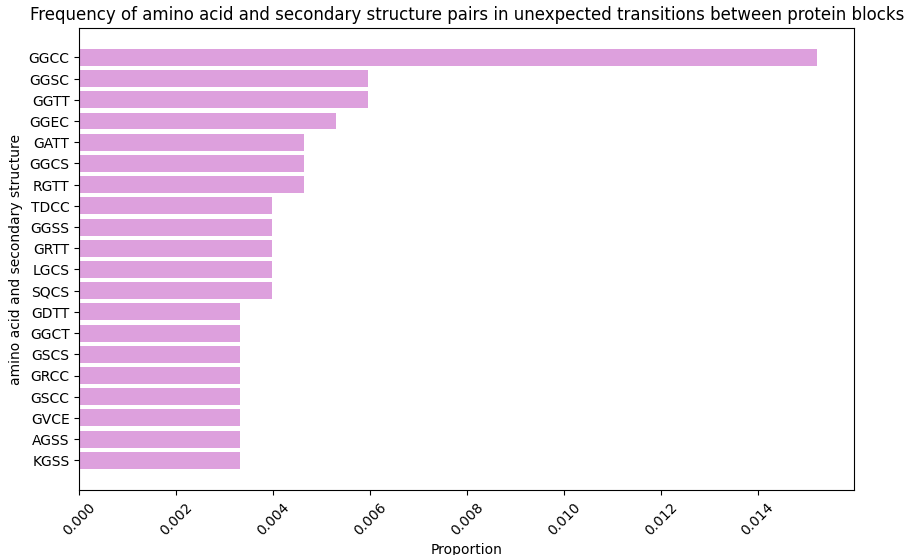
\includegraphics[width=1\textwidth]{./images/aas2freq.png}
    \caption{Frekvencija kombinacija parova aminokiselina i sekundarnih struktura u retkim prelazima.}
    \label{Slika:aas2freq}
\end{figure}
\\
Rezultati pokazuju da je daleko najzastupljenija kombinacija GG CC. Može se zaključiti da je razlog toga visok stepen fleksibilnosti glicina, koji ga može učiniti sklonijim ka formiranju neregularnih konformacija. Prethodna analiza je pokazala da su pojedinačno najzastupljeniji parovi aminokiselina i sekundarnih struktura baš glicin i neregularno stanje, što dodatno doprinosi tvrdnji da postoji visoka korelisanost kako između njih tako i između njih i proteinskih blokova koji čine prelaz.\\
Sve kombinacije parova aminokiselina i sekundarnih strukura, zajedno sa njihovim frekvencijama, sačuvani su u datoteci \\\texttt{amino\_acid\_secondary\_structure\_combination.csv}.
\subsection{Analiza vrednosti pLDDT parametra}
pLDDT (\textit{eng. the predicted local distance difference test}) predstavlja meru pouzdanost lokalne strukture proteina, predviđene AlphaFold2 programom. Vrednosti su na skali od 0 do 100, pri čemu veće vrednosti ukazuju na visoku pouzdanost i precizniju predikciju. \\
Vrednosti pLDDT veće od 90 se kategorišu kao najveća preciznost i tada se smatra da su i kičma i bočni lanci proteina predviđeni sa visokom preciznošću. Nasuprot tome, vrednosti ispod 70 tipično ukazuju na ispravno predviđenu kičmu, ali sa mogućim greškama u predikciji bočnih lanaca. \\
Važno je napomenuti da pLDDT vrednost može značajno varirati duž proteinskog lanca. S obzirom da se ova mera odnosi se na pojedinačne regione strukture, određeni segmenti mogu biti predviđeni s visokom pouzdanošću, dok drugi mogu imati nisku prediktivnu tačnost. \\
Niska pLDDT vrednost u određenim oblastima proteina može biti posledica više faktora. Najčešći uzroci su visoka fleksibilnost regiona ili odsustvo dobro definisane strukture. Takođe, moguće je da oblast ima stabilnu strukturu, ali da nedostaju relevantni podaci neophodni za pouzdanu predikciju pomoću AlphaFold2 programa. U oba slučaja, ovakvim oblastima se obično pridružuje pLDDT vrednost ispod 50.\\ 
Na slici \ref{Slika:plddt} prikazan je primer strukture proteina sa određenim pLDDT vrednostima.
\begin{figure}[htbp]
    	\centering
    	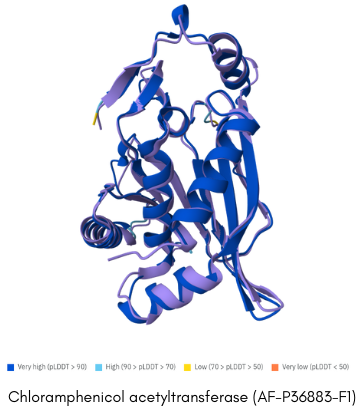
\includegraphics[width=0.7\textwidth]{./images/plddt.png}
    	\caption{Prosečna pLDDT vrednost za protein Chloramphenicol acetyltransferase iznosi 96.28.}
    	\label{Slika:plddt}
\end{figure}
\\
Glavni cilj ovog dela analize je upravo bio ispitivanje prirode vrednosti pLDDT mere u podacima.
\newpage
\subsubsection{Srednja vrednost pLDDT parametra u podacima}
Ispitivanje srednje vrednosti pLDDT podrazumeva analiziranje vrednosti ove mere na celom skupu podataka. Ovakva analiza omogućava donošenje zaključaka o preciznosti predikcija lokalnih struktura proteina čiji su proteinski blokovi bili predmet intraživanja u ovom radu. \\
Radi utvrđivanja prirode posmatrane mere, najpre je konstruisan histogram vrednosti pLDDT. Prikaz histograma je dat na slici \ref{Slika:distribution}.
\begin{figure}[htbp]
    	\centering
    	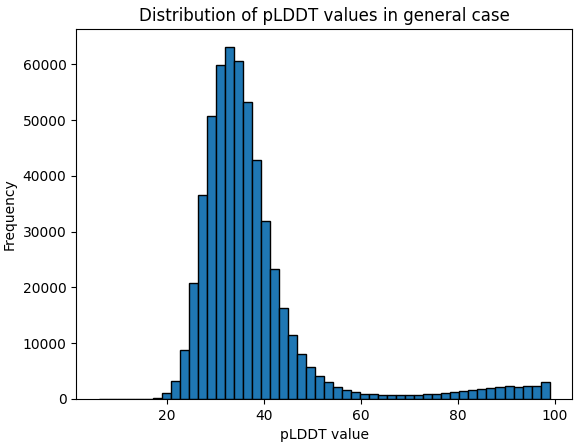
\includegraphics[width=0.8\textwidth]{./images/dist_dataset.png}
    	\caption{Histogram raspodele pLDDT vrednosti u celom skupu podataka}
    	\label{Slika:distribution}
\end{figure}
\\
Raspodela pokazuje izraženu asimetričnost, sa dominantnim vrhom u intervalu 30–40 i dugim desnim repom. Ovakav oblik raspodele sugeriše da može biti aproksimirana gama raspodelom ili nekom drugom asimetričnom raspodelom. Dodatno, primećuje se manja frekvencija pLDDT vrednosti u višem opsegu (iznad 70), što može ukazivati na retkost visoko pouzdanih predikcija u opštem slučaju. \\
Za preciznije ispitivanje raspodele, potrebno je izračunati osnovne opisne statistike. Srednja vrednost iznosi približno 37.6, 0.75 kvantil 39.6, dok maksimalna pLDDT vrednost koja se javlja u skupu iznosi 98.95. Vrednost ostalih statistika dat je u tabeli \ref{Tabela:4}.
\begin{table}[h!]
    \centering
    \begin{tabular}{ |l|l| } 
    \hline
    \textbf{Opisna statistika} & \textbf{pLDDT} \\
    \hline
    mean & 37.586782 \\
    std  & 13.145442 \\
    min  & 5.920000 \\
    $25\%$  & 30.540001 \\
    $50\%$   & 34.570000 	\\
    $75\%$ & 39.570000 	 \\
    max & 98.949997 	\\
    \hline
    \end{tabular}
    \caption{Osnovne opisne statistike za pLDDT parametar.}
    \label{Tabela:4}
\end{table}
\newpage
Zaključak je da se u podacima najčešće javljaju veoma niske pLDDT vrednosti. Ovaj rezultat može da sugeriše na to da analizu nije prikladno vršiti na osnovu celih redova u skupu podataka zbog potencijalne pristrasnosti vrednostima koje se javljaju samo u određenim prelazima, za određene proteine. Iz tog razloga, potrebno je grupisati podatke na osnovu nekog atributa i dalje vršiti analizu.
\subsubsection{Vrednosti pLDDT prema proteinskim blokovima}
Sledeći korak analize pLDDT-a jeste ispitivanje vrednosti te mere u odnosu na proteinske blokove. Ispitivanje je vršeno tako što su se podaci grupisali na osnovu parova proteinskih blokova. Nakon toga, izračunata je prosečna vrednost pLDDT mere. Na taj način dodeljena je reprezentativna pLDDT vrednost za svaki par proteinskih blokova. \\
Ideja je da se za određeni prelaz utvrdi da li se pretežno javljaju visoke ili niske vrednosti pLDDT-a i na taj način donese zaključak da li taj prelaz sadrži relativno precizno predviđene lokalne strukture proteina. \\
Da bi se dobila relevantna informacija o prirodi vrednosti pLDDT u odnosu na sve prelaze, izračunate su opisne statistike za tako grupisane podatke. Pregled vrednosti statistika je dostupan u tabeli \ref{Tabela:5}.
\begin{table}[h!]
    \centering
    \begin{tabular}{ |l|l| } 
    \hline
    \textbf{Opisna statistika} & \textbf{pLDDT} \\
    \hline
    mean & 63.454415 \\
    std  & 18.023050 \\
    min  & 33.597163 \\
    $25\%$  & 45.888131 \\
    $50\%$  & 65.646074 	\\
    $75\%$ &  79.848490\\
    max & 90.566951 	\\
    \hline
    \end{tabular}
    \caption{Osnovne opisne statistike za pLDDT parametar prema proteinskim blokovima.}
    \label{Tabela:5}
\end{table}

Prosečna vrednost od približno 63.45 ukazuje na to da, posmatrano u odnosu na parove proteinskih blokova, pLDDT vrednost teži visoko pouzdanoj. Takođe, izračunat je broj parova kod kojih se javlja visoka vrednost. Dobijeno je da se u 49 od 106, odnosno u $46.23\%$, retkih prelaza između proteinskih blokova dostiže precizna predikcija lokalne strukture proteina. U tabeli \ref{Tabela:6} dat je prikaz parova proteinskih blokova za koje se vezuju veoma visoke vrednosti pLDDT-a. U tim prelazima nisu prisutni proteinski blokovi g, h, ni kao par, ni pojedinačno, dok se i i j javljaju ali veoma retko i ne zajedno. S obzirom na to da oni odgovaraju nespecifičnim strukturama (eng. \textit{coil–coil}), opravdano je da se za njih vezuju niže vrednosti pLDDT-a.
\begin{table}[h!]
\centering
\begin{tabular}{|c|c|c|}
\hline
\textbf{PB1} & \textbf{PB2} & \textbf{pLDDT} \\
\hline
n & k & 90.57 \\
\hline
f & o & 90.30 \\
\hline
p & n & 88.73 \\
\hline
k & p & 88.16 \\
\hline
i & m & 87.34 \\
\hline
m & j & 87.13 \\
\hline
d & n & 85.99 \\
\hline
e & n & 85.81 \\
\hline
k & i & 85.79 \\
\hline
e & l & 85.53 \\
\hline
\end{tabular}
\caption{Parovi proteinskih blokova (PB1-PB2) sa najvišom prosečnom vrednošću pLDDT-a.}
\label{Tabela:6}
\end{table}

Sve vrednosti parametra \texttt{pLDDT} u odnosu na proteinske blokove sačuvane su u datoteci \texttt{plDDT\_protein\_block.csv}.
\subsubsection{Vrednosti pLDDT prema aminokiselinama}
U ovom delu analize podaci su grupisani na osnovu parova aminokiselina, izračunata je prosečna vrednost pLDDT mere za svaki par i na kraju određene opisne statistike, date u tabeli \ref{Tabela:7}.
\begin{table}[h!]
    \centering
    \begin{tabular}{ |l|l| } 
    \hline
    \textbf{Opisna statistika} & \textbf{pLDDT} \\
    \hline
    mean & 38.670799 \\
    std  & 3.802211 \\
    min  & 33.752673 \\
    $25\%$  & 36.140094 \\
    $50\%$  & 37.688579 	\\
    $75\%$ & 39.974417\\
    max & 61.994733 	\\
    \hline
    \end{tabular}
    \caption{Osnovne opisne statistike za pLDDT parametar prema aminokiselinama.}
    \label{Tabela:7}
\end{table}

Dobijeni rezultati ukazuju na veoma niske vrednosti posmatrano prema parovima aminokiselina. Maksimalna vrednost u skupu pokazuje da se ni za jedan par ne javljaju visoko pouzdane vrednosti, odnosno vrednosti iznad 70. Naime, razlog ovako niskih vrednosti leži u tome što ista kombinacija aminokiselina može da se pojavi u potpuno različitim delovima različitih proteina, i to u okruženjima sa različitom stabilnošću, fleksibilnošću i strukturnom definisanošću što dovodi do velike varijacije pLDDT vrednosti.\\
Sve vrednosti parametra \texttt{pLDDT} u odnosu na aminokiseline sačuvane su u datoteci \texttt{plDDT\_amino\_acid.csv}.
\subsubsection{Vrednosti pLDDT prema sekundarnim strukturama}
U analizi pLDDT mere ostalo je još ispitati njene vrednosti u odnosu na parove sekudarnih struktura. Ispitivanje je vršeno identično kao u slučaju parova proteinskih blokova i aminokiselina - podaci su najpre grupisani, zatim je izračunata prošečna pLDDT vrednost i na kraju su izračunate vrednosti statistika za novoformirani skup podataka koje su date u tabeli \ref{Tabela:8}.
\begin{table}[h!]
    \centering
    \begin{tabular}{ |l|l| } 
    \hline
    \textbf{Opisna statistika} & \textbf{pLDDT} \\
    \hline
    mean & 73.448625 \\
    std  & 15.828469 \\
    min  & 35.300866 \\
    $25\%$  & 65.967828 \\
    $50\%$  & 78.462409 	\\
    $75\%$ & 85.288241\\
    max & 95.586667 	\\
    \hline
    \end{tabular}
    \caption{Osnovne opisne statistike za pLDDT parametar prema sekundarnim strukturama.}
    \label{Tabela:8}
\end{table}

Vrednosti opisnih statistika, pre svega prosečna vrednost od približno 73.45 i medijana od približno 78.46, ukazuju na visoku pouzdanost u ovom slučaju. Takođe, čak $68.97\%$, odnosno 40 od 58, parova sekundarnih struktura ima pLDDT vrednost iznad 70. Može se zaključiti da većinu parova, u prelazima čiji su deo, odlikuje precizna predikcija strukture. U tabeli \ref{Tabela:9} izvojeni su oni parovi kod kojih se javljaju najviše pLDDT vrednosti.
\begin{table}[h!]
\centering
\begin{tabular}{|c|c|c|}
\hline
\textbf{S2\_1} & \textbf{S2\_2} & \textbf{pLDDT} \\
\hline
B & E & 95.59 \\
\hline
B & H & 95.20 \\
\hline
G & E & 92.51 \\
\hline
H & E & 92.51 \\
\hline
T & B & 88.82 \\
\hline
S & E & 88.16 \\
\hline
E & C & 87.04 \\
\hline
S & B & 86.99 \\
\hline
G & H & 86.99 \\
\hline
E & E & 86.85 \\
\hline
\end{tabular}
\caption{Parovi sekundarnih struktura (S2\_1 - S2\_2) sa najvišom prosečnom vrednošću pLDDT-a.}
\label{Tabela:9}
\end{table}
\newpage
Najpouzdaniji parovi sekundarnih struktura, odnosno parovi čija pLDDT vrednost prelazi 90, uglavnom uključuju elemente B, E i H, što je očekivano jer upravo ovi oblici strukture predstavljaju najstabilnije i najčešće strukturne oblike u proteinima. Odnosno, sasvim je prirodno pretpostaviti da će AlphaFold2 program moći baš te najosnovnije sekundarne strukture da predvidi precizno.\\
Sve vrednosti parametra \texttt{pLDDT} u odnosu na sekundarne strukture sačuvane su u datoteci \texttt{plDDT\_secondary\_structure.csv}.
\subsection{Analiza vrednosti RSA parametra}
Pored pLDDT parametra, od posebnog interesa za analizu je bio i parametar RSA (eng. \textit{relative solvent accessibility}). RSA predstavlja meru izloženosti aminokiselinskog ostatka rastvaraču (vodi) u strukturi proteina i koristi se za opisivanje biofizičkih karakteristika proteina. Vrednost RSA za aminokiselinski ostatak računa se na osnovu formule:
\begin{equation}
\text{RSA} = \frac{\text{ASA}}{\text{maxASA}}
\end{equation}
gde je \textit{ASA} (eng. \textit{accessibility surface area}) pristupačna površina rastvaraču, a \textit{maxASA} maksimalna moguća pristupačna površina rastvaraču za datu aminokiselinu. \\
Na osnovu vrednosti RSA, odnosno izračunatoj izloženosti rastvaraču, aminokiselinski ostaci mogu biti „zakopani” (eng. \textit{buried}) ili „izloženi” (eng. \textit{exposed}). Definicije praga za klasifikaciju aminokiselina u jednu od dve kategorije variraju, međutim, u većini slučajeva prag se definiše kao $25\%$ vrednosti RSA, odnosno ukoliko aminokiselinski ostatak ima vrednost RSA manju od $25\%$ onda se može zaključiti da on nije izložen rastvaraču (zakopan), u suprotnom je izložen \cite{wu2020rsa}. S obzirom na to da je prag relativno mali, potrebno je razumeti da vrednosti iznad praga označavaju različite stepene izloženosti rastvaraču. Naime, vrednosti iznad $90\%$ ukazuju na to da je ostatak gotovo čitavom površinom dostupan rastvaraču i istraživanja pokazuju da se takve konformacije najčešće javljaju u petljama (eng. \textit{loops}) i okretima (\textit{turns}) \cite{tien2013maxasa}, dok vrednosti bliže $25\%$ označavaju blagu izloženost tj. izloženost manjih delova površine ostatka. Na slici \ref{Slika:rsa} prikazane su 3D strukture proteina proteina glutamin sintaze i K-Ras-a sa izračunatim RSA vrednostima za neke aminokiselinske ostatke. 
\begin{figure}[htbp]
    \centering
    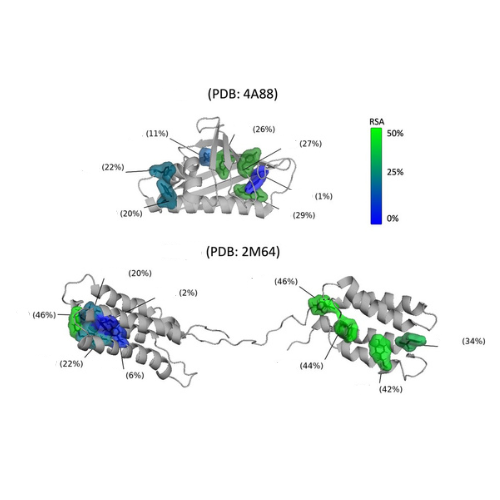
\includegraphics[width=0.9\textwidth]{./images/rsa.png}
    \caption{RSA vrednosti za aminokiselinske ostatke u proteinima.}
    \label{Slika:rsa}
\end{figure}
\\
\subsubsection{Srednja vrednost RSA parametra u podacima}
Radi utvrđivanja RSA vrednosti u skupu podataka izračunate su opisne statistike i određen je broj izloženih i zakopanih aminokiselinskih ostataka. U podacima postoje dve kolone koje se odnose na RSA jer se svaki prelaz između proteinskih blokova sastoji od para aminokiselina za koji je određena RSA vrednost. U skladu sa tim, prilikom računanja brojnosti svake od RSA kategorija sabrane su vrednosti dobijene za prvu i drugu kolonu. \\
Za obe kolone dobijena je srednja vrednost od približno $92\%$, dok medijana i treći kvartil iznose $100\%$. Takođe, dobijeno je da je $97.5\%$ aminokiselinskih ostataka, posmatrano u opštem slučaju, izloženo. Zaključak je da su u podacima daleko zastupljenije izložene aminokiseline i to visoko izložene, odnosno tako da su gotovo čitavom površinom dostupne rastvaraču.
\subsubsection{Vrednosti RSA prema proteinskim blokovima}
U ovom delu analize, podaci najpre grupisani na osnovu prelaza između proteinskih blokova, analogno pristupu koji je korišćen u analizi parametra pLDDT. Budući da za svaki prelaz postoje dve RSA vrednosti (po jedna za svaki od dva susedna ostatka), izračunata je njihova prosečna vrednost, koja je potom dodeljena kao reprezentativna vrednost za dati prelaz. Nad tako grupisanim podacima izračunate su opisne statistike, čije vrednosti su date u tabeli \ref{Tabela:10}.
\begin{table}[h!]
    \centering
    \begin{tabular}{ |l|l| } 
    \hline
    \textbf{Opisna statistika} & \textbf{RSA} \\
    \hline
    mean & 64.219617 \\
    std  & 20.352375 \\
    min  & 22.983397 \\
    $25\%$  & 48.298345 \\
    $50\%$  & 59.209232 	\\
    $75\%$ & 83.560475\\
    max & 96.876662 	\\
    \hline
    \end{tabular}
    \caption{Osnovne opisne statistike za RSA parametar prema proteinskim blokovima.}
    \label{Tabela:10}
\end{table}

Rezultati ukazuju da su aminokiselinski ostaci, posmatrano za svaki pojedinačni prelaz, srednje izloženi rastvaraču odnosno da se nalaze u umereno izloženim regijama strukture. Posebno je značajan podatak da se kod čak $99.06\%$ svih prelaza beleži prosečna RSA vrednost iznad $25\%$, što sugeriše da se potpuno zakopane aminokiseline praktično ne javljaju kao karakteristika celih parova proteinskih blokova, već eventualno samo lokalno, na nivou pojedinačnih ostataka. \\
Sve vrednosti parametra \texttt{RSA} u odnosu na proteinske blokove sačuvane su u datoteci \texttt{RSA\_protein\_block.csv}.
\subsubsection{Vrednosti RSA prema aminokiselinama}
Za potrebe detaljnije analize, izvršeno je i ispitivanje prirode vrednosti RSA prema parovima aminokiselina u prelazima. Primenjena metodologija je identična kao u prethodnoj analizi – podaci su grupisani prema svim mogućim parovima aminokiselina koji se javljaju u prelazima, a zatim je za svaki par izračunata prosečna vrednost RSA. Na tako grupisanim podacima izračunate su osnovne opisne statistike prikazane u Tabeli \ref{Tabela:11}.
\begin{table}[h!]
    \centering
    \begin{tabular}{ |l|l| } 
    \hline
    \textbf{Opisna statistika} & \textbf{RSA} \\
    \hline
    mean & 89.822263 \\
    std  & 5.541973 \\
    min  & 65.555131 \\
    $25\%$  & 65.555131 \\
    $50\%$  & 90.880001 	\\
    $75\%$ & 93.854497\\
    max & 98.135047 	\\
    \hline
    \end{tabular}
    \caption{Osnovne opisne statistike za RSA parametar prema aminokiselinama.}
    \label{Tabela:11}
\end{table}

Rezultati pokazuju izuzetno visoku prosečnu izloženost aminokiselinskih parova, sa srednjom vrednošću od približno $90\%$, što znači da se velika većina analiziranih parova nalazi u izloženim regijama proteinskih struktura. Čak i prvi kvartil iznosi $65.56\%$, što implicira da ni u jednom od posmatranih parova aminokiselina ne dolazi do značajnije zaklonjenosti površine.\\
Sve vrednosti parametra \texttt{RSA} u odnosu na aminokiseline sačuvane su u datoteci \texttt{RSA\_amino\_acid.csv}.
\subsubsection{Vrednosti RSA prema sekundarnim strukturama}
Na kraju ove analize, ispitana je pristupačnost aminokiselinskih ostataka rastvaraču u kontekstu parova sekundarnih struktura koje definišu prelaz. Kao i u prethodnim slučajevima, podaci su grupisani na osnovu para, izračunata je prosečna RSA vrednost i određene su potrebne statistike za analiziranje prirode RSA vrednosti. Rezultati su dati u tabeli \ref{Tabela:12}.
\begin{table}[h!]
    \centering
    \begin{tabular}{ |l|l| } 
    \hline
    \textbf{Opisna statistika} & \textbf{RSA} \\
    \hline
    mean & 41.925664 \\
    std  & 30.019328 \\
    min  & 0.000000 \\
    $25\%$  & 16.518614 \\
    $50\%$  & 43.529417 	\\
    $75\%$ & 62.653578\\
    max & 97.473198 	\\
    \hline
    \end{tabular}
    \caption{Osnovne opisne statistike za RSA parametar prema sekundarnim strukturama.}
    \label{Tabela:12}
\end{table}

Dobijeni rezultati ukazuju na širi raspon izloženosti aminokiselinskih ostataka u zavisnosti od kombinacije sekundarnih struktura u prelazu. Srednja vrednost i medijana impliciraju umerenu izloženost u većini slučajeva. \\
Zanimljivo je da je $58.62\%$ svih analiziranih parova sekundarnih struktura imalo prosečnu RSA vrednost veću od $25\%$, što ukazuje da je više od polovine parova locirano u regijama koje su bar delimično dostupne rastvaraču. S druge strane, prisustvo prelaza sa RSA vrednostima bliskim nuli ukazuje na to da neki tipovi sekundarnih struktura uključuju strukturno zaklonjene pozicije. \\
Sve vrednosti parametra \texttt{RSA} u odnosu na sekundarne strukture sačuvane su u datoteci \texttt{RSA\_secondary\_structure.csv}.
\subsection{Ispitivanje zastupljenosti aminokiselina u podacima}

Kodon je triplet nukleotida, odnosno tri uzastopna nukleotida mRNK. Kodoni predstavljaju šifre za aminokiseline. Jedna aminokiselina može biti kodirana jednim kodonom ili sa više kodona. Aminokiseline se dalje kombinuju i kreiraju proteine. Postoje regioni u kodu proteina gde sastav aminokiselina nije od značaja, i gde se neke aminokiseline pojavljuju više od drugih. Postavlja se pitanje da li je to slučajno ili postoji neki razlog koji objašnjava prezastupljenost određenih aminokiselina. 
Određivanje prezastupljenosti i podzastupljenosti aminokiselina vršeno je poređenjem frekvencije aminokiseline u podacima sa očekivanim vrednostima frekvencija. Očekivane vrednosti frekvencije  kodona računaju se množenjem prirodnih frekvencija svake DNK baze koja čini kodon, gde se frekvencije u prirodi za uracil 22\%, citozin 21.7\%, guanin 26.1\% i adeninn 30.3\%. Zatim se očekivana vrednost frekvencije aminokiseline dobija kao suma očekivanih vrednosti svih kodona koji kodiraju tu aminokiselinu. Kako postoje tri kodona koji ne kodiraju aminokiseline već su stop ili nonsense kodoni, prethodnu sumu treba pomnožiti faktorom korekcije 1.057. \cite{nimbios_aminoacid}


\begin{table}[htbp]
    \centering
    \resizebox{\textwidth}{!}{
    \begin{tabular}{|c|c|c|}
        \hline
        \textbf{Aminokiseline} & \textbf{Kodoni} & \textbf{Posmatrana zastupljenost kod kičmenjaka} \\
        \hline
        Alanine & GCU, GCA, GCC, GCG & 7.4\% \\ \hline
        Arginine & CGU, CGA, CGC,CGG, AGA, AGG & 4.2\%  \\ \hline
        Asparagine & AAU, AAC & 4.4\% \\ \hline
        Aspartic Acid & GAU, GAC & 5.9\% \\ \hline
        Cysteine & UGU, UGC & 3.3\% \\ \hline
        Glutamic Acid & GAA, GAG & 5.8\% \\ \hline
        Glutamine & CAA, CAG & 3.7\% \\ \hline
        Glycine & GGU, GGA, GGC, GGG & 7.4\% \\ \hline
        Histidine & CAU, CAC & 2.9\% \\ \hline
        Isoleucine & AUU, AUA, AUC & 3.8\% \\ \hline
        Leucine & CUU, CUA, CUC, CUG, UUA, UUG & 7.6\% \\ \hline
        Lysine & AAA, AAG & 7.2\% \\ \hline
        Methionine & AUG & 1.8\% \\ \hline
        Phenylalanine & UUU, UUC & 4.0\% \\ \hline
        Proline & CCU, CCA, CCC, CCG & 5.0\% \\ \hline
        Serine & UCU, UCA, UCC, UCG, AGU, AGC & 8.1\% \\ \hline
        Threonine & ACU, ACA, ACC, ACG & 6.2\% \\ \hline
        Tryptophan & UGG & 1.3\% \\ \hline
        Tyrosine & UAU, UAC & 3.3\% \\ \hline
        Valine & GUU, GUA, GUC, GUG & 6.8\% \\ \hline
        Stop Codons & UAA, UAG, UGA & --- \\ \hline
    \end{tabular}
    }
    \caption{Posmatrana zastupljenost aminokiselina kod kičmenjaka}
    \label{Tabela:13}
\end{table}

Posmatrane frekvencije aminokiselina izračunate su prebrojavanjem svih aminokiselina koje se javljaju u prelazima, računajući i atribut AA1 i atribut AA2, i njihovim deljenjem sa ukupnim brojem prelaza.
Na slici \ref{Slika:aafreq.barplot} su prikazane učestalosti aminokiselina u posmatranom uzorku (plavo) i njihove
očekivane vrednosti prema referentnoj raspodeli (narandžasto). Uočava se da određene
aminokiseline značajno odstupaju od očekivanih vrednosti. Posebno se izdvaja serin (S),
koji je u uzorku zastupljen više od 40\% iznad reference. Pored njega, povećanu učestalost
pokazuju i glutaminska kiselina (E), glicin (G), lizin (K), arginin (R) i treonin (T).  

S druge strane, neke aminokiseline su ređe zastupljene nego što se očekuje, među njima
cistein (C), izoleucin (I), leucin (L), valin (V) i tirozin (Y).  

Ovi rezultati ukazuju da uzorak može biti pristrasan ka fleksibilnim i polarnim
aminokiselinama (poput S i G), kao i ka naelektrisanim aminokiselinama (E, K, R).

\begin{figure}[htbp]
    \centering
    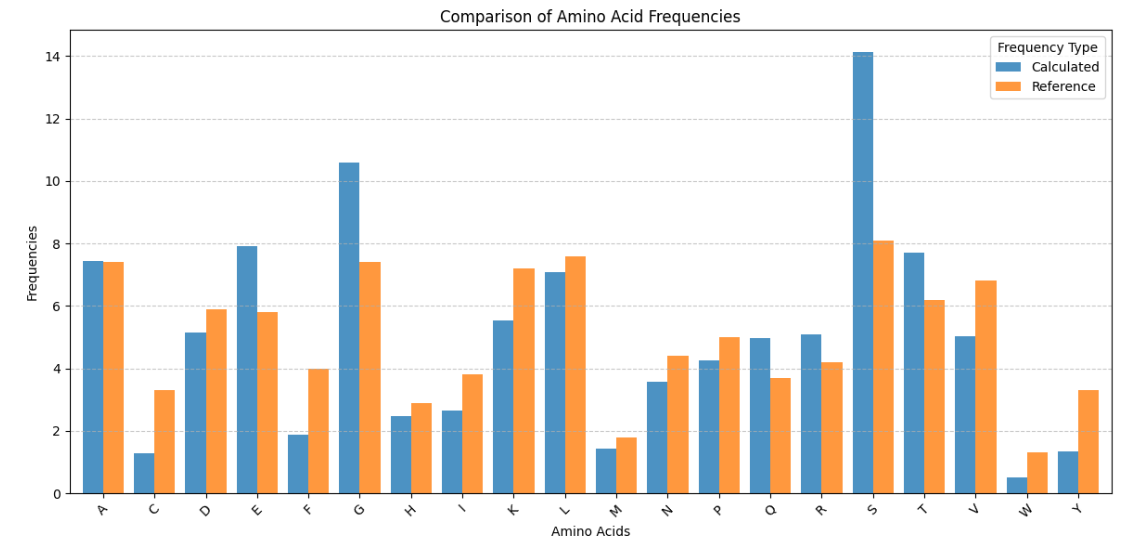
\includegraphics[width=1\textwidth]{./images/aafreq.barplot.png}
    \caption{Poređenje izračunatih i referentnih zastupljenosti aminokiselina}
    \label{Slika:aafreq.barplot}
\end{figure}

\begin{figure}[htbp]
    \centering
    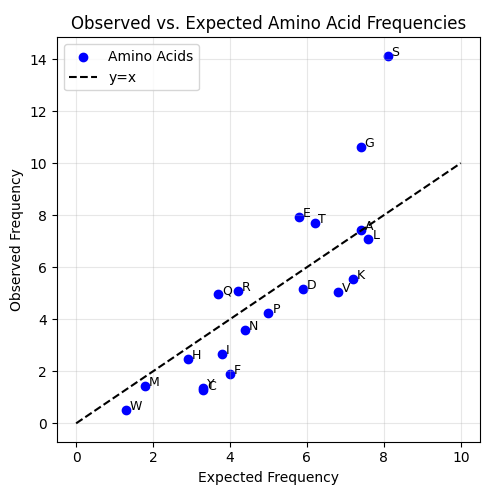
\includegraphics[width=0.6\textwidth]{./images/obsvsexp.png}
    \caption{Poređenje izračunatih i referentnih zastupljenosti aminokiselina}
    \label{Slika:obsvsexp}
\end{figure}


\newpage
\section{Klasifikacija}
Algoritmi klasifikacije se u mašinskom učenju koriste za predviđanje ciljnog atributa, klase, na osnovu ostalih atributa. U našem primeru vršimo klasifikaciju za tri različite ciljne promenljive, parove aminokiselina, parove sekundarnih struktura i parove proteinskih blokova na prelazima.

Kako se bavimo prelazima i parovima na njima najpre je neophodno da izvršimo konkatenaciju određenih kolona i napravimo novu kolonu koja će služiti kao ciljna promenljiva. Vrednosti iz prve i druge kolone su konkatenirane uz očuvanje redosleda (npr. 'jb' nije isto što i 'bj').

\subsection{Balansiranost klasa}
Kod problema klasifikacije podataka važno je proveriti balansiranost klasa, odnosno da li se sve klase ravnomerno javljaju ili postoje neke koje su zastupljenije. U slučaju da postoje klase koje su značajno brojnije od drugih može doći do pristrasnosti tim klasama i zanemarivanju ređih klasa, što dovodi do lošije preciznosti modela.
Kako je postoji 20 aminokiselina, a mi predviđamo parove aminokiselina, ukupan broj klasa je 20*20 = 400. Na slici \ref{Slika:aa_imbalance} predstavljena je raspodela klasa aminokiselina.
Kao što se može videti na slici, distribucija učestalosti ovih klasa pokazuje izrazitu nebalansiranost. Većina primera pripada manjem broju najčešćih klasa, dok veliki broj kombinacija ima relativno mali broj instanci, pa čak i ispod 100 ponavljanja. Posebno je izazovno u ovom slučaju to što se radi o velikom broju klasa (400), što dodatno otežava balansiranje i evaluaciju.
\\
\begin{figure}[htbp]
    \centering
    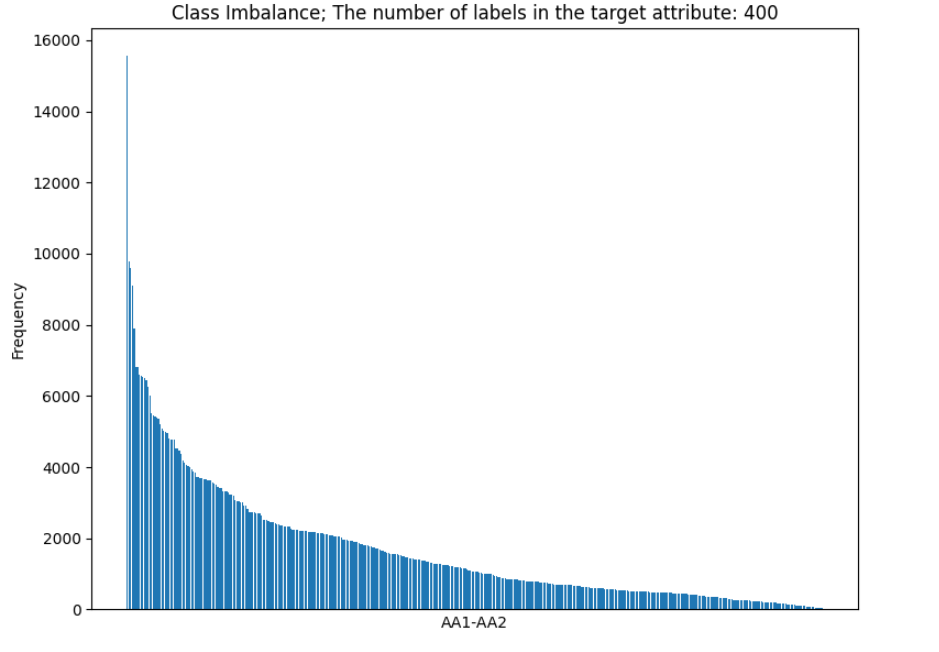
\includegraphics[width=1\textwidth]{./images/aa_imbalance.png}
    \caption{Balansiranost klasa za parove aminokiselina.}
    \label{Slika:aa_imbalance}
\end{figure}

U slučaju kada je ciljna promenljiva kombinacija parova proteinskih blokova, kojih u skupu podataka ima ukupno 152, histogram prikazuje izrazitu nebalansiranost u raspodeli ovih klasa (Slika \ref{Slika:pb_imbalance}). Nekoliko najfrekventnijih kombinacija pojavljuje se i preko 100.000 puta, dok se velika većina ostalih klasa javlja sa znatno manjom učestalošću, od nekoliko stotina do čak ispod 100.
\begin{figure}[htbp]
    \centering
    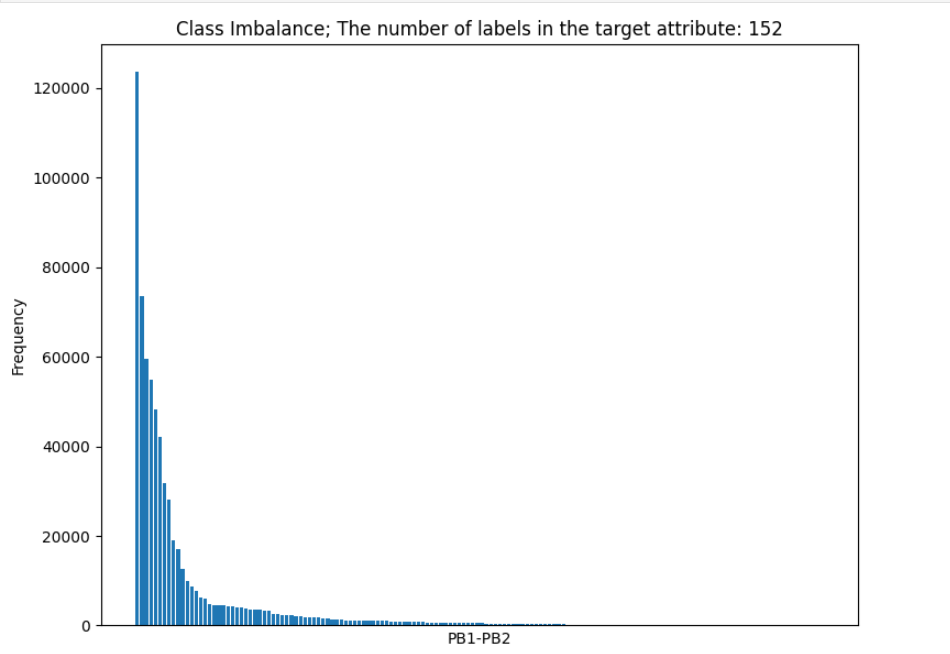
\includegraphics[width=1\textwidth]{./images/pb_imbalance.png}
    \caption{Balansiranost klasa za parove proteinskih blokova.}
    \label{Slika:pb_imbalance}
\end{figure}

U slučaju kombinacija sekundarnih struktura, pri čemu je ukupno identifikovano 65 različitih kombinacija, vizuelna analiza raspodele klasa (prikazana na slici \ref{Slika:ss_imbalance}) ukazuje na ekstremnu nebalansiranost. Jedna jedina klasa dominira skupom sa preko 500.000 instanci, dok su ostale klase višestruko manje zastupljene — mnoge sa frekvencijom manjom od 10.000, a neke i blizu nule.

\begin{figure}[htbp]
    \centering
    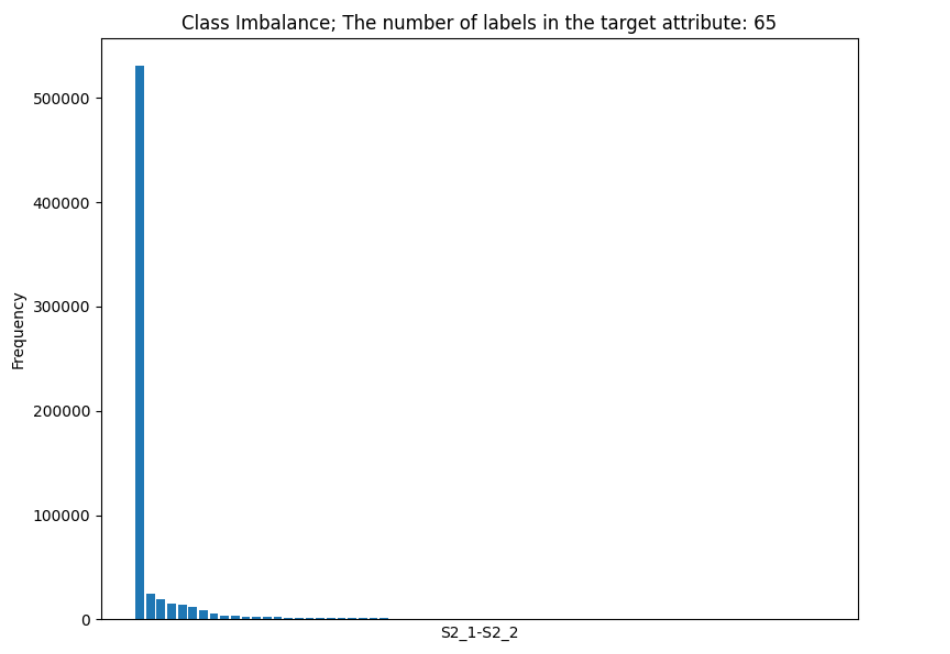
\includegraphics[width=1\textwidth]{./images/ss_imbalance.png}
    \caption{Balansiranost klasa za parove sekundarnih struktura.}
    \label{Slika:ss_imbalance}
\end{figure}
\newpage
Ovakva distribucija je tipična za biološke podatke, gde određene strukturne konfiguracije imaju prirodno dominantniju ulogu. Međutim, iz perspektive učenja modela, ovolika razlika u broju primera po klasi može izazvati značajnu pristrasnost prilikom treniranja klasifikatora, jer dominantna klasa može preuzeti "težinu" u učenju i prouzrokovati značajnu pristrasnost modela, čime se tačnost predikcija za ređe klase drastično smanjuje. U takvom okruženju, model koji samo predviđa najčešću klasu može imati visoku ukupnu tačnost, ali loše performanse na nivou klasa, što se posebno vidi u metrikama kao što su \textit{recall}.
\newpage

\subsection{CatBoost}

CatBoost je savremeni algoritam za mašinsko učenje baziran na gradijentnom buđenju stabala (eng. gradient boosting on decision trees), razvijen od strane kompanije Yandex. Osmišljen je sa ciljem da poboljša efikasnost i tačnost u radu sa strukturisanim podacima, posebno u scenarijima gde su prisutne i numeričke i kategorijske promenljive. Za razliku od drugih popularnih implementacija kao što su XGBoost i LightGBM, CatBoost ima ugrađenu podršku za direktno korišćenje kategorijskih promenljivih bez potrebe za njihovom prethodnom transformacijom u numerički format (npr. putem one-hot enkodiranja), čime se pojednostavljuje priprema podataka i smanjuje mogućnost preprilagođavanja.
Prilikom treniranja modela korišćen je parametar \texttt{auto\_class\_weights=\textquotesingle Balanced\textquotesingle}, koji omogućava CatBoost algoritmu da automatski izračuna težine za svaku klasu na osnovu njihove učestalosti u skupu podataka. Ova tehnika se koristi za ublažavanje uticaja nebalansiranosti klasa, pri čemu ređe klase dobijaju veću težinu tokom treniranja, čime se smanjuje pristrasnost modela prema češće zastupljenim klasama.

Težina $w_i$ za svaku klasu $i$ računa se po sledećoj formuli:

\[
w_i = \frac{N}{k \cdot N_i}
\]

gde je:
\begin{itemize}
    \item $N$ --- ukupan broj primera u skupu podataka,
    \item $k$ --- broj različitih klasa,
    \item $N_i$ --- broj primera koji pripadaju klasi $i$.
\end{itemize}

\subsubsection*{Aminokiseline}

Rezultati pokazuju izuzetno nisku tačnost, odziv (recall) i F1-meru na test i trening skupu, dok je preciznost (precision) relativno visoka ($\sim$0.63). Ovo može ukazivati na neravnotežu klasa u skupu podataka, gde model nauči da klasifikuje samo dominantnu klasu.

\bigskip
\begin{itemize}
    \item \textbf{Tačnost (Accuracy)} je niska na oba skupa ($\sim$2--2.5\%), što znači da je model uspešan samo u malom broju slučajeva.
    \item \textbf{Odziv (Recall)} je takođe nizak, što znači da model propušta većinu pozitivnih primera.
    \item \textbf{Preciznost (Precision)} je relativno visoka --- kada god model klasifikuje neku instancu kao pozitivnu, uglavnom je u pravu, ali to radi vrlo retko.
\end{itemize}
S obzirom da su metrike na trening i test skupu veoma slične, možemo zaključiti da nema značajnog preprilagođavanja. Model se ponaša jednako loše na oba skupa.

\begin{table}[h!]
    \centering
    \caption{Evaluacija modela na test i trening skupu za parove aminokiselina}
    \begin{tabular}{l|cc}
    \textbf{Metrička vrednost} & \textbf{Test skup} & \textbf{Trening skup} \\
    \hline
    Tačnost (Accuracy)   & 0.0227   & 0.0255 \\
    Preciznost (Precision) & 0.6285   & 0.6292 \\
    Odziv (Recall)        & 0.0227   & 0.0255 \\
    F1 mera (F1 Score)     & 0.0103   & 0.0122 \\
    \end{tabular}
\end{table}

\begin{figure}[htbp]
    \centering
    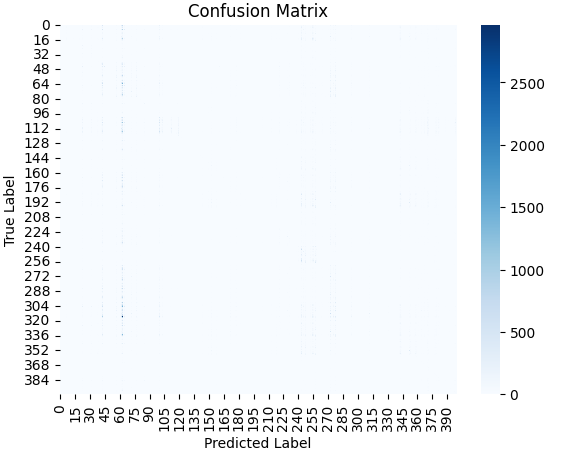
\includegraphics[width=0.8\textwidth]{./images/conf_mat_aa.png}
    \caption{Matrica konfuzije za parove aminokiselina.}
    \label{Slika:confmataa}
\end{figure}

\subsubsection*{Proteinski blokovi}

Rezultati pokazuju da model ostvaruje visoku tačnost, odziv, F1-meru i preciznost na oba skupa, što ukazuje na efikasnu klasifikaciju proteinskih blokova. Vrednosti metrika su gotovo identične na test i trening skupu, što znači da nema izraženog preprilagođavanja.


\begin{table}[h!]
\centering
\caption{Evaluacija modela na test i trening skupu za parove proteinskih blokova}
\begin{tabular}{l|cc}
\textbf{Metrička vrednost} & \textbf{Test skup} & \textbf{Trening skup} \\
\hline
Tačnost (Accuracy)     & 0.9418 & 0.9427 \\
Preciznost (Precision) & 0.9606 & 0.9613 \\
Odziv (Recall)         & 0.9418 & 0.9427 \\
F1 mera (F1 Score)     & 0.9472 & 0.9481 \\
\end{tabular}
\end{table}


\begin{itemize}
    \item \textbf{Tačnost (Accuracy)} je visoka ($\sim$94.2\%) na oba skupa, što ukazuje na generalno uspešnu klasifikaciju većine uzoraka.
    \item \textbf{Preciznost (Precision)} i \textbf{odziv (Recall)} su uravnoteženi, što znači da model uspešno prepoznaje većinu pozitivnih primera, uz minimalan broj lažnih pozitivnih.
    \item \textbf{F1 mera} potvrđuje ravnotežu između odziva i preciznosti.
\end{itemize}

\bigskip


\begin{figure}[htbp]
    \centering
    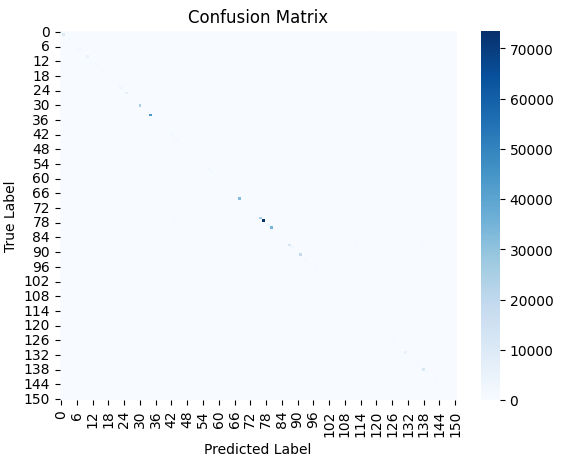
\includegraphics[width=0.8\textwidth]{./images/conf_mat_pb.png}
    \caption{Matrica konfuzije za parove proteinskih blokova.}
    \label{Slika:confmatpb}
\end{figure}


\subsubsection*{Sekundarne strukture}

Prikazane metrike modela na test i trening skupu ukazuju na umereno dobar učinak, sa značajnim neskladom između preciznosti i odziva (recall).

\begin{table}[h!]
\centering
\caption{Evaluacija modela na test i trening skupu za parove }
\begin{tabular}{l|cc}
\textbf{Metrička vrednost} & \textbf{Test skup} & \textbf{Trening skup} \\
\hline
Tačnost (Accuracy)     & 0.4251 & 0.4252 \\
Preciznost (Precision) & 0.8489 & 0.8488 \\
Odziv (Recall)         & 0.4251 & 0.4252 \\
F1 mera (F1 Score)     & 0.5540 & 0.5536 \\
\end{tabular}
\end{table}

\bigskip

Rezultati pokazuju da model ima visoku preciznost ($\sim0.85$), što znači da je većina klasifikacija pozitivnih primera tačna, ali je odziv (recall) nizak ($\sim0.43$), što ukazuje da model propušta veliki broj stvarnih pozitivnih primera.

\begin{itemize}
    \item \textbf{Tačnost (Accuracy)} od oko 42.5\% ukazuje na umereno dobru ukupnu preciznost klasifikacije.
    \item \textbf{Nesklad između visoke preciznosti i niskog odziva} može ukazivati na neuravnoteženost klasa ili na to da model često izostavlja pozitivne slučajeve.
    \item \textbf{F1 mera} od oko 0.55 pokazuje da postoji prostor za poboljšanje u balansu između preciznosti i odziva.
\end{itemize}
S obzirom da su metrike na test i trening skupu veoma slične, nema indikacija o značajnom preprilagođavanju.

\begin{figure}[htbp]
    \centering
    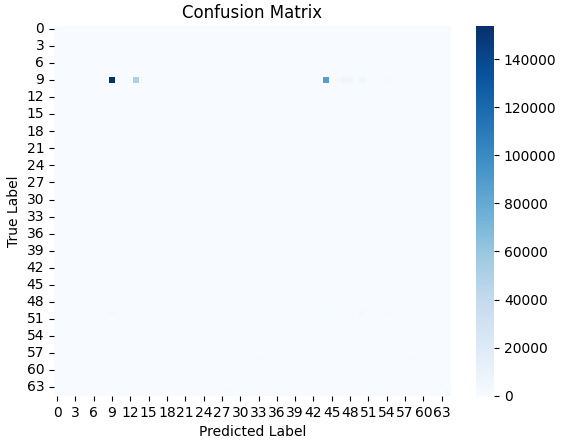
\includegraphics[width=0.8\textwidth]{./images/conf_mat_ss.png}
    \caption{Matrica konfuzije za parove sekundarnih struktura.}
    \label{Slika:confmatss}
\end{figure}

\subsection{Neuronske mreže}

Neuronske mreže predstavljaju klasu modela koji se inspirišu strukturom i funkcionisanjem bioloških neuronskih sistema. Njihova moć ogleda se u sposobnosti da modeluju kompleksne i nelinearne odnose u podacima, što ih čini pogodnim za širok spektar zadataka u klasifikaciji, regresiji i obradi nestrukturiranih podataka. Posebno su uspešne u višeklasnoj klasifikaciji, pod uslovom da je ulazni prostor pravilno pripremljen.

\subsubsection*{Priprema podataka}
Ciljna promenljiva, koja je inicijalno sadržila kategoričke oznake klasa, transformisana je u numeričke vrednosti korišćenjem klase \texttt{LabelEncoder} iz biblioteke \texttt{scikit-learn}. Ova transformacija omogućava jednoznačno mapiranje svake klase na pripadajuću celobrojnu oznaku.

Ulazne promenljive podeljene su na numeričke i kategoričke kolone. Kategoričke promenljive su kodirane tehnikom \textit{One-Hot} kodiranja, gde se svaka diskretna vrednost reprezentuje binarnim vektorom. Numeričke kolone su standardizovane tako da imaju nultu srednju vrednost i jediničnu standardnu devijaciju, čime se obezbeđuje ujednačen doprinos svih numeričkih osobina.

Zbog izražene nebalansiranosti među klasama ciljne promenljive, bilo je neophodno primeniti metod za balansiranje. Korišćena je funkcija \\ \texttt{compute\_class\_weight} sa parametrom \texttt{'balanced'}, koja automatski izračunava težine svake klase inverzno proporcionalno njenoj učestalosti u skupu za trening. Dobijene težine se kasnije prosleđuju modelu kao dodatni parametar kako bi se kompenzovala prekomerna zastupljenost dominantnih klasa i omogućilo pravičnije učenje.

\subsubsection*{Formiranje modela}

Model veštačke neuronske mreže konstruisan je korišćenjem biblioteke \texttt{Keras}, sa ciljem klasifikacije podataka u više klasa. Arhitektura modela sastoji se od dva skrivena sloja, pri čemu prvi sloj sadrži 128, a drugi 64 neurona, oba sa ReLU aktivacionom funkcijom. Radi smanjenja mogućnosti preprilagođavanja (\textit{overfitting}), između slojeva su uključeni Dropout slojevi sa stopom izostavljanja od 30\%. Izlazni sloj koristi \texttt{softmax} aktivacionu funkciju, što omogućava višeklasnu klasifikaciju.
\\
Model je kompajliran korišćenjem Adam optimizatora sa unapred definisanom brzinom učenja, dok je funkcija greške bila \texttt{categorical\_crossentropy}, što je standardni izbor za probleme višeklasne klasifikacije. Kao mera uspešnosti modela korišćena je tačnost (\textit{accuracy}).

Radi poboljšanja performansi modela, sprovedena je ručna pretraga hiperparametara (engl. \textit{manual grid search}). Istraživane su različite vrednosti broja neurona u skrivenim slojevima, stope izostavljanja (dropout), kao i vrednosti stope učenja. Evaluacija svakog modela u okviru pretrage vršena je na osnovu tačnosti na validacionom skupu, čime je odabran skup hiperparametara koji daje najbolje rezultate.

\subsubsection*{Aminokiseline}

\begin{figure}[htbp]
    \centering
    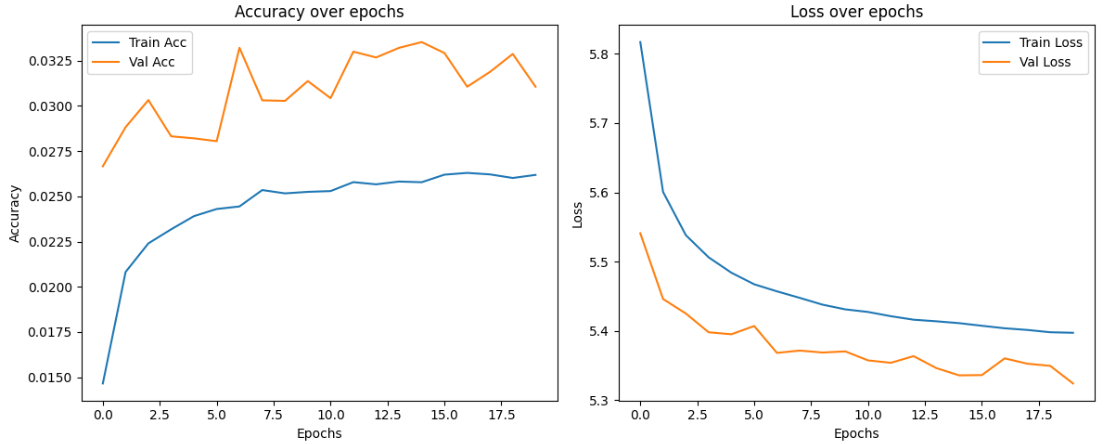
\includegraphics[width=1\textwidth]{images/epochs_aa.png}
    \caption{Prikaz preciznosti (levo) i gubitka (desno) tokom epoha za najbolji model pronađen Grid pretragom}
    \label{fig:accuracy_loss}
\end{figure}

Na slici \ref{fig:accuracy_loss} prikazana je promena tačnosti i funkcije greške modela tokom 20 epoha treniranja. Može se uočiti da se tačnost modela na trening skupu postepeno povećava, dok se vrednost funkcije greške smanjuje, što ukazuje na uspešno učenje modela. Takođe, validacioni rezultati pokazuju sličan trend: preciznost na validacionom skupu ostaje viša od one na trening skupu, što sugeriše da model generalizuje dobro i ne pokazuje jasne znake preprilagođavanja (engl. \textit{overfitting}) u ovom broju epoha.

Ipak, apsolutne vrednosti preciznosti su niske (ispod 4\%), što ukazuje na izazovnost klasifikacionog problema i moguću potrebu za dodatnim unapređenjem modela, kao što su optimizacija arhitekture, izbor relevantnijih osobina ili balansiranje skupa podataka na drugi način. S obzirom na veliku neravnotežu među klasama i veliki broj klasa, ovakvi rezultati su očekivani i zahtevaju dublju analizu distribucije podataka.

\subsubsection*{Proteinski blokovi}

\begin{figure}[htbp]
    \centering
    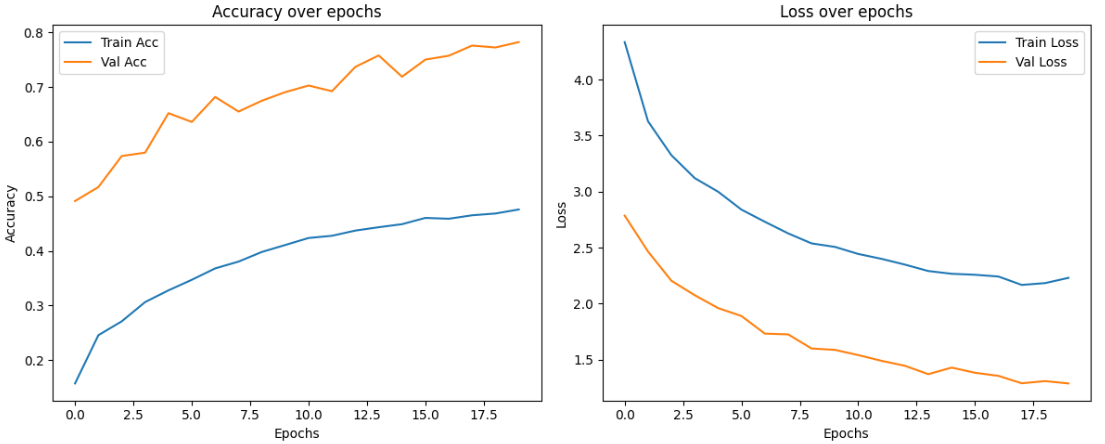
\includegraphics[width=1\textwidth]{images/epochs_pb.png}
    \caption{Preciznost (levo) i funkcija greške (desno) tokom epoha za klasifikaciju proteinskih blokova}
    \label{fig:pb_accuracy_loss}
\end{figure}

Na slici \ref{fig:pb_accuracy_loss} prikazani su rezultati treniranja neuronske mreže za klasifikaciju proteinskih blokova. Model pokazuje jasan trend poboljšanja kako u pogledu tačnosti, tako i u pogledu smanjenja funkcije greške. Tačnost na trening skupu konstantno raste, dok se vrednosti funkcije greške smanjuju, što je očekivano ponašanje tokom treniranja.

Zanimljivo je da model postiže znatno bolju tačnost na validacionom skupu (preko 75\% u poslednjim epohama), nego na trening skupu (oko 47\%).

Trendovi funkcije greške pokazuju da validacioni gubitak brzo opada i stabilizuje se, dok trening gubitak opada sporije, što ukazuje na stabilno učenje bez znakova preprilagođavanja (engl. \textit{overfitting}) u posmatranom intervalu epoha.

Ovi rezultati sugerišu da je zadatak klasifikacije proteinskih blokova uspešnije rešiv u odnosu na klasifikaciju aminokiselinskih parova, što može biti posledica boljih ulaznih reprezentacija, većih razlika među klasama ili manje izražene nebalansiranosti skupa podataka.

\subsubsection*{Sekundarne strukture}

\begin{figure}[htbp]
    \centering
    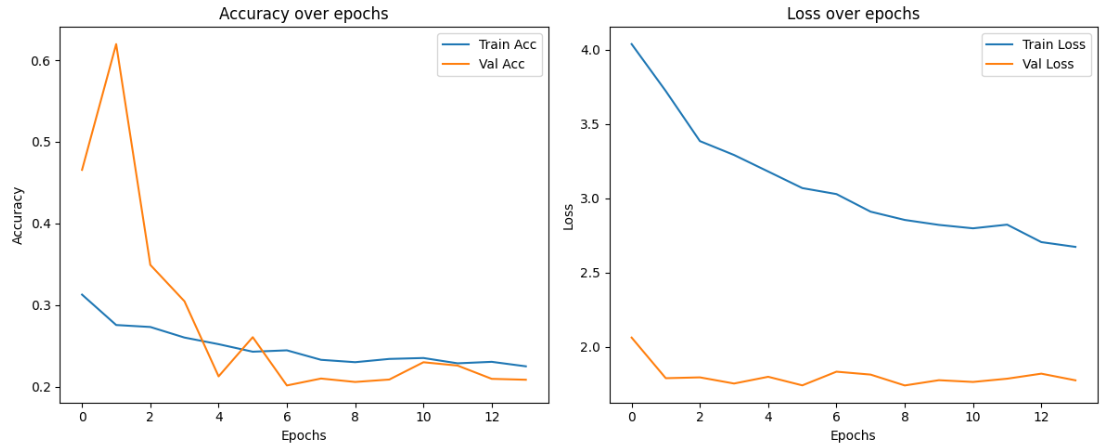
\includegraphics[width=1\textwidth]{images/epochs_ss.png}
    \caption{Preciznost (levo) i funkcija greške (desno) tokom epoha za klasifikaciju sekundarnih struktura}
    \label{fig:ss_accuracy_loss}
\end{figure}

Na slici \ref{fig:ss_accuracy_loss} prikazano je praćenje tačnosti i vrednosti funkcije greške tokom epoha treniranja modela za klasifikaciju sekundarnih struktura. Za razliku od prethodnih zadataka, ovde je uočen nestabilan obrazac u metrikama validacije, preciznost validacionog skupa varira značajno kroz epohe, bez jasnog trenda poboljšanja, dok vrednosti gubitka ostaju gotovo konstantne posle početnog pada.

S druge strane, trening metrika pokazuje blagi pad greške i stabilnu, ali relativno nisku tačnost. Ovakvi rezultati mogu ukazivati na nekoliko potencijalnih problema: visoka složenost samog zadatka, izražena klasa nebalansiranost ili manjak reprezentativnosti validacionog skupa.

\newpage
\section{Klasterovanje}
Klasterovanje predstavlja postupak grupisanja podataka na osnovu međusobne sličnosti, pri čemu se formiraju grupe tj. klasteri unutar kojih su podaci najsličniji jedni drugima. U mašinskom učenju postoji veliki broj algoritama klasterovanja u zavisnosti od prirode podataka. U ovom radu, predmet analize je skup podataka sa mešovitim tipovima atributa. Kategorički atributi odnose se na parove proteinskih blokova, aminokiselina i sekundarnih struktura, dok numerički atributi obuhvataju očekivanu učestalost prelaza između proteinskih blokova, pLDDT vrednosti i RSA parametre. Dakle, cilj ovog dela rada jeste da se izvrši klasterovanje prelaza između proteinskih blokova.

S obzirom na karakteristike podataka, izbor algoritama pogodnih za njihovo grupisanje je ograničen. Stoga je za potrebe ovog istraživanja odabran algoritam \textit{K-Prototypes}, koji je specijalizovan za rad sa mešovitim podacima i omogućava istovremeno korišćenje različitih mera sličnosti za numeričke i kategoričke atribute.

\subsection{K-Prototypes}
K-Prototypes algoritam predstavlja proširenje dobro poznatog K-means algoritma - koji radi samo sa numeričkim podacima, i njegove varijante za čisto kategoričke podatke K-modes.
\\ Razvijen je s ciljem klasterovanja mešovitih podataka. Ovakvi podaci zahtevaju specifičan pristup, jer tradicionalne mere sličnosti nisu podjednako pogodne za oba tipa atributa.
\\ K-Prototypes koristi kombinovanu meru sličnosti kojom integriše Euklidsko rastojanje za numeričke atribute i jednostavno uparivanje koeficijenata (SMC - sample matching coefficient) za kategoričke atribute:

\begin{itemize}
    \item \textbf{Numerički atributi:} Sličnost se meri pomoću standardnog Euklidskog rastojanja:
    \[
    d_{num}(x_i, z_l) = \sum_{j=1}^{m_r} (x_{ij}^{(r)} - z_{lj}^{(r)})^2
    \]
    gde je $l$ indeks posmatranog klastera, $r$ oznaka da je u pitanju numerički atribut, $x_{ij}^{(r)}$ vrednost $j$-tog numeričkog atributa instance (tačke) $i$, a $z_{lj}^{(r)}$ odgovarajuća vrednost prototipa(centra) klastera $l$ za atribut $j$. U ovom slučaju centar predstavlja aritmetičku sredinu svih tačaka u tom klasteru.

    \item \textbf{Kategorički atributi:} Različitost se izražava kroz broj nepodudaranja između kategoričkih vrednosti:
    \[
    d_{cat}(x_i, z_l) = \gamma \sum_{j=1}^{m_c} \delta(x_{ij}^{(c)}, z_{lj}^{(c)})
    \]
    gde je $\delta(x, z) = 0$ ako su vrednosti jednake, a $1$ ako nisu. Koeficijent $\gamma$ predstavlja težinu kategoričkih atributa u ukupnoj meri različitosti.
    
\end{itemize}
Ukupna udaljenost između instance $x_i$ i prototipa $z_l$ definisana je kao:
\[
d(x_i, z_l) = \sum_{j=1}^{m_r} (x_{ij}^{(r)} - z_{lj}^{(r)})^2 + \gamma \sum_{j=1}^{m_c} \delta(x_{ij}^{(c)}, z_{lj}^{(c)})
\]

Cilj K-Prototypes algoritma jeste minimizacija ukupne funkcije cene (engl. \textit{cost function}), koju je definisao Huang. Ukupna funkcija cene sastoji se iz dve komponente: troška za numeričke atribute i troška za kategoričke atribute:

\[
Cost = \sum_{l=1}^{k} \sum_{x_i \in C_l} \left( \sum_{j=1}^{m_r} (x_{ij}^{(r)} - z_{lj}^{(r)})^2 + \gamma \sum_{j=1}^{m_c} \delta(x_{ij}^{(c)}, z_{lj}^{(c)}) \right)
\]

gde je:
\begin{itemize}
    \item $k$ broj klastera,
    \item $C_l$ skup instanci dodeljenih klasteru $l$,
    \item $m_r$ broj numeričkih atributa,
    \item $m_c$ broj kategoričkih atributa,
    \item $z_l$ centar klastera $l$.
\end{itemize}
Minimizacijom ukupne funkcije cene (\textit{eng. cost}) postiže se optimalno grupisanje instanci u klastere koji su međusobno što sličniji unutar klastera, a što različitiji između klastera. Uzimajući u obzir i numeričke i kategoričke atribute u istoj formuli, K-Prototypes predstavlja robustan i efikasan pristup klasterovanju mešovitih podataka i zato je izabran u ovom radu.
\subsection{Vizuelizacija podataka}
Budući da K-Prototypes algoritam zahteva unapred definisan broj klastera, vizuelizacija podataka može biti korisna pomoć pri određivanju odgovarajuće vrednosti ovog parametra. S obzirom na to da skup podataka koji se klasteruje sadrži deset atributa, odnosno da je višedimenzionalan, za svrhe prikaza podataka u dve dimenzije neophodno je primeniti neku od tehnika redukcije dimenzionalnosti.

U ovom radu izabrana je tehnika \textbf{UMAP} (\textit{eng. Uniform Manifold Approximation and Projection}).
\subsubsection{UMAP}
UMAP je nelinearna metoda redukcije dimenzionalnosti koja se zasniva na matematičkim principima i oblastima kao što su Rimanova geometrija i algebarska topologija. Osmišljena je da očuva lokalnu i globalnu strukturu podataka prilikom projekcije u niži dimenzionalni prostor. Osim očuvanja globalne strukture prednosti UMAP-a se ogledaju i u skalabilnosti (podržava efikasan rad sa velikim skupovima podataka) i fleksibilnosti (pored vizuelizacije koristi se i u opšte svrhe redukcije dimenzionalnosti).

Zbog sposobnosti da efikasno obradi velike i kompleksne skupove podataka mešovitog tipa, kao i da prepozna nelinearne obrasce, UMAP se pokazao kao prikladan alat za otkrivanje potencijalne strukture klastera u primeru konrektnog skupa podataka koji se koristi u radu.

Za potrebe ove analize korišćena je implementacija iz biblioteke \texttt{umap-learn} u \textit{Python}-u. Zbog veličine originalnog skupa podataka (preko 670.000 redova) i njegove kompleksnosti (kombinacija kategoričkih atributa sa puno vrednosti i numeričkih atributa), izvršeno je slučajno uzorkovanje od 10\% instanci radi ubrzanja procesa. Numerički atributi su prethodno transformisani korišćenjem \texttt{Yeo-Johnson} transformacije radi stabilizacije disperzije i približavanja normalnoj raspodeli, dok su kategorički atributi enkodirani uz pomoć \texttt{LabelEncoder}-a. Tako pripremljeni podaci su zatim prosleđeni UMAP algoritmu radi vizuelizacije u dvodimenzionalnom prostoru. \footnote{Parametri \texttt{n\_components=2}, \texttt{n\_neighbors=10} i \texttt{min\_dist=0.3} određuju dimenziju prikaza, broj suseda za lokalno modeliranje i minimalnu međusobnu udaljenost tačaka u projektovanom prostoru, respektivno.}

Na slici \ref{Slika:umap} prikazan je rezultat UMAP vizuelizacije.
\newpage
\begin{figure}[htbp]
    	\centering
    	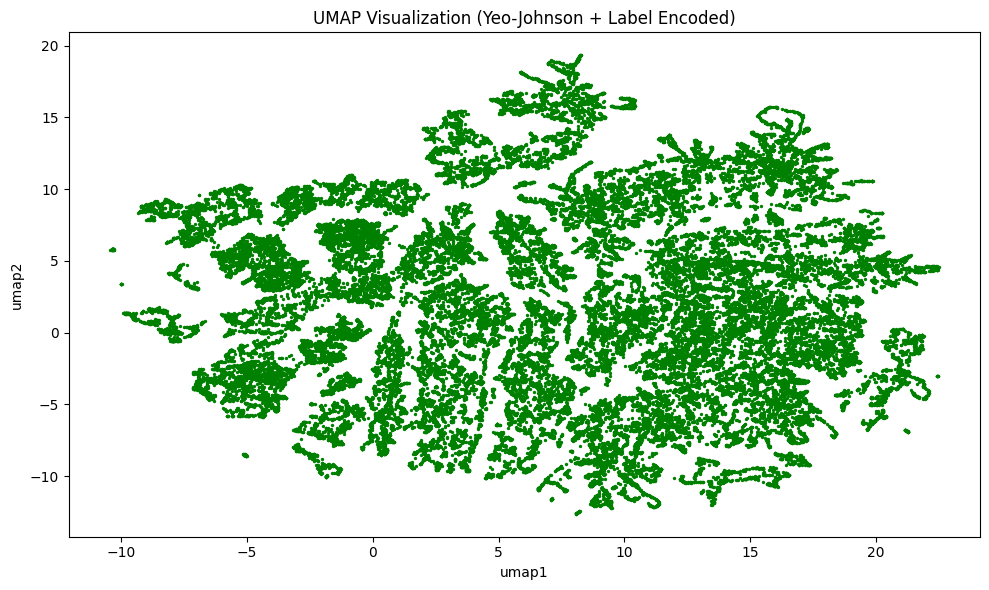
\includegraphics[width=1\textwidth]{./images/umap.png}
    	\caption{UMAP vizualizacija podataka (Yeo-Johnson + Label Encoding)}
    	\label{Slika:umap}
\end{figure}

Na osnovu dobijene UMAP projekcije može se uočiti da postoje relativno jasno odvojene grupe tačaka, što vizuelno ukazuje na postojanje klastera u podacima. Ipak, treba imati u vidu da je projekcija urađena na ograničenom uzorku podataka pa se broj uočenih grupa ne mora u potpunosti preslikavati na ceo skup. 

Analizom rezultata vizualizacije, odlučeno je da se klasterovanje detaljnije ispita za vrednosti broja klastera $k = 8$ i $k = 10$, kako bi se obuhvatile najistaknutije strukture u podacima.
\subsection{Pretprocesiranje podataka}
Pre primene K-Prototypes algoritma, neophodno je sprovesti odgovarajuće korake pripreme podataka, imajući u vidu da ovaj algoritam istovremeno obrađuje numeričke i kategoričke atribute.
\\
Za numeričke atribute, izvršena je standardizacija pomoću \texttt{StandardScaler} iz biblioteke \texttt{sklearn}, čime se postiže da svi atributi imaju srednju vrednost 0 i standardnu devijaciju 1. Ova transformacija je važna kako bi se numerički atributi nalazili na uporedivoj skali i kako bi se sprečilo da atributi sa većim numeričkim rasponom dominiraju u računanju sličnosti.
\\
Za kategoričke atribute, dodatna transformacija nije neophodna jer \\K-Prototypes koristi internu reprezentaciju za poređenje kategoričkih vrednosti. Međutim, neophodno je obezbediti indeksne pozicije kolona koje predstavljaju kategoričke atribute, kako bi ih algoritam mogao prepoznati.

\subsection{Rezultati klasterovanja}
Algoritam \texttt{K-Prototypes} primenjen je nad celokupnim skupom podataka, koji sadrži ukupno $671{,}155$ instanci i $10$ atributa mešovitog tipa (numeričkih i kategoričkih). Klasterovanje je sprovedeno za dva različita broja klastera -- $k=8$ i $k=10$, kako bi se omogućilo poređenje rezultata i procena optimalnog broja klastera.

Za $k=8$, dobijena ukupna cena klasterovanja (\texttt{cost\_}) iznosi približno \textbf{1.392.549}, dok za $k=10$ iznosi nešto niže, približno \textbf{1.316.788}, što ukazuje na nešto bolje interno uklapanje instanci u klastere kod većeg broja klastera.

Radi vizuelne interpretacije rezultata, odnosno prikaza klastera, iskorišćena je UMAP tehnika nad uzorkom od $10\%$ celokupnog skupa podataka. Vizuelizacija 8 klastera je prikazana na slici \ref{Slika:clusters1}, dok slika \ref{Slika:clusters2} predstavlja vizuelizaciju 10 klastera.

\begin{figure}[htbp]
    	\centering
    	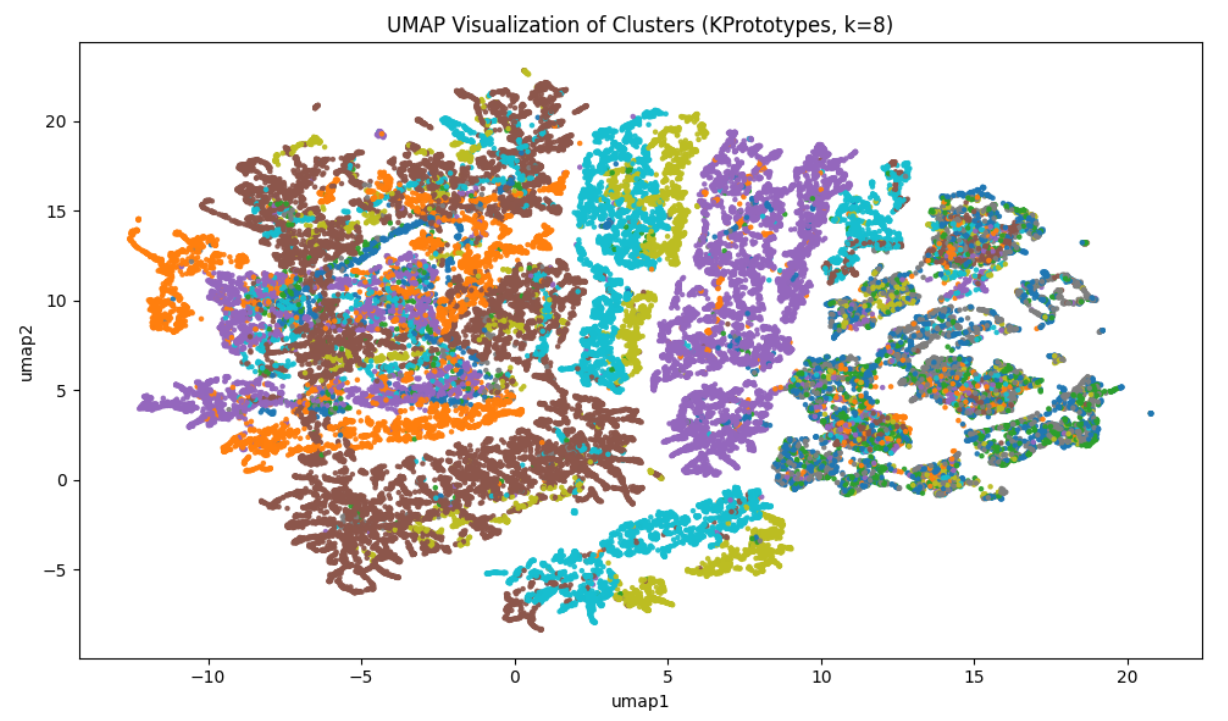
\includegraphics[width=1\textwidth]{./images/umap_clusters1.png}
    	\caption{Vizuelizacija klastera (k=8)}
    	\label{Slika:clusters1}
\end{figure}
\begin{figure}[htbp]
    	\centering
    	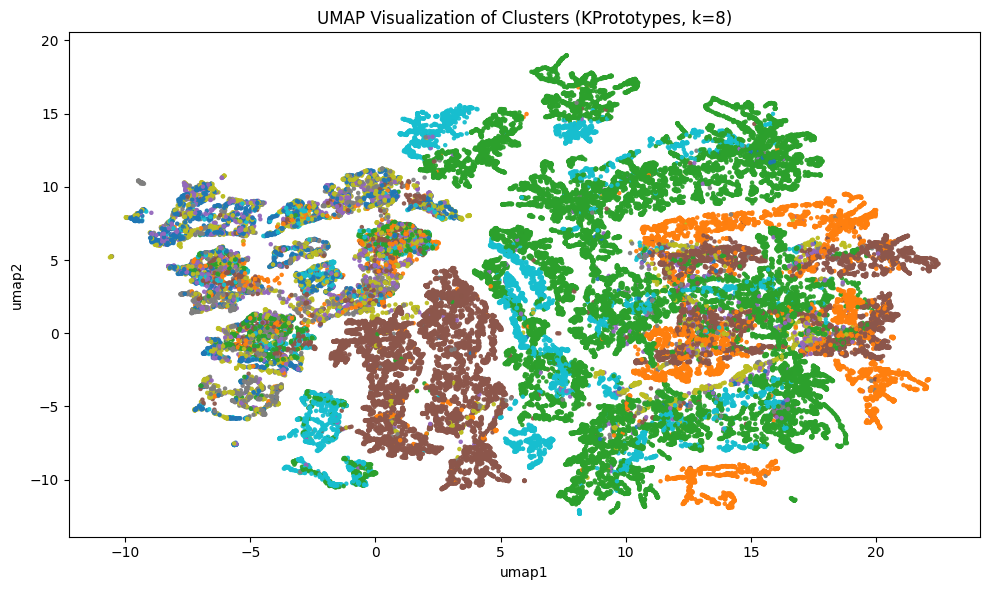
\includegraphics[width=1\textwidth]{./images/umap_clusters2.png}
    	\caption{Vizuelizacija klastera (k=10)}
    	\label{Slika:clusters2}
\end{figure}

Procena kvaliteta klasterovanja izvršena je pomoću senka koeficijenta \textit{eng. silhouette coefficient}, prilagođenog za mešovite tipove podataka korišćenjem \textbf{Gower} rastojanja. Zbog veličine skupa podataka i formiranja matrice prilikom računanja \textbf{Gower} rastojanja, evaluacija je sprovedena nad uzorkom od 4\%. 

Dobijeni rezultati su sledeći:
\begin{itemize}
    \item Za $k=8$ vrednost senka koeficijent iznosi \textbf{0.1663}.
    \item Za $k=10$ vrednost senka koeficijent iznosi \textbf{0.1682}.
\end{itemize}

Obe vrednosti ukazuju na slabo izraženu, ali prisutnu strukturu klastera i delimičnu odvojenost klastera. Nešto viši rezultat za $k=10$ sugeriše da veći broj klastera može bolje obuhvatiti varijacije u podacima. Međutim, treba imati u vidu da se evaluacija vršila na uzorku.

Iz rezultata se zaključuje da među prelazima proteinskih blokova postoji izvesna sličnost, ali ona nije jasno izražena u prostoru karakteristika.
\newpage
\section{Zaključak}
Cilj ovog rada bila je sveobuhvatna analiza prelaza između proteinskih blokova radi razumevanja njihove strukturne i funkcionalne uloge u opisu trodimenzionalne strukture proteina.\\
\\
Analitički deo je ukazao na to da je par (glicin, glicin) daleko najzastupljeniji par aminokiselina u prelazima, što potvrđuje njegovu povezanost sa fleksibilnošću u proteinskoj strukturi i dovodi do zaključka da u prelazima postoji stabilnost. Sekundarne strukture koje dominiraju u prelazima su neregularne strukture C (\textit{eng. coil}), S ({\textit{eng. bend}), T ({\textit{eng. helix turn}}). Analiza vrednosti pLDDT i RSA parametara prema svakoj od struktura u prelazu omogućila je procenjivanje pouzdanosti predikcije prelaza i izloženosti rastvaraču, pri čemu su najpouzdanija predviđanja vezana za stabilne sekundarne strukture poput $\alpha$-zavojnica i $\beta$-ploča dok su aminokiseline u prelazima pokazale izuzetno visoku prosečnu izloženost rastvaraču.\\
\\
U okviru klasifikacije, CatBoost i neuronske mreže pokazale su značajno bolje rezultate u predikciji proteinskih blokova, gde CatBoost ostvaruje visoku tačnost, odziv, F1-meru i preciznost (vrednosti svih metrika imaju vrednost preko 90\%), u odnosu na aminokiseline i sekundarne strukture.\\
\\
Klasterovanje algoritmom K-Prototypes pokazalo je postojanje određene, ali slabije izražene strukture među prelazima, čime je potvrđena složenost podataka i heterogenost njihovih karakteristika. Vizuelizacija pomoću UMAP-a omogućila je identifikaciju potencijalnih klastera, dok je modifikovan senka koeficijent (\textit{eng. silhouette coefficient}) nad uzorkom podataka ukazao na delimičnu odvojenost klastera.\\
\\
Rad zaključuje da proteinski blokovi kao strukturni alfabeti predstavljaju koristan model za analizu lokalnih struktura proteina. Iako postoje izazovi u klasifikaciji i jasnom grupisanju zbog prirode podataka, kombinacija opisne i prediktivne analize omogućava detaljno sagledavanje uloge pojedinačnih struktura u prelazima i njihovih međusobnih odnosa.

\newpage
\begin{thebibliography}{5}
    \bibitem{carter2003dsspcont} 
    Phil Carter, Claus A. F. Andersen, Burkhard Rost. 
    \textit{DSSPcont: Continuous Secondary Structure Assignments for Proteins}. 
    Bioinformatics, 19(2):230-231, 2003.
    \bibitem{dong2012glycines}
    Hao Dong, Mukesh Sharma, Huan-Xiang Zhou, Timothy A. Cross.  
    \textit{Glycines: Role in $\alpha$-Helical Membrane Protein Structures and a Potential Indicator for Native Conformation}.  
    Biochemistry, 51(26): 5299-5307, 2012.  
    PMCID: PMC3426646, NIHMSID: NIHMS383776, PMID: 22650985.
    \bibitem{debrevern2010proteinblocks} 
    Agnel Praveen Joseph, Garima Agarwal, Swapnil Mahajan, 
    Jean-Christophe Gelly, Lakshmipuram S. Swapna, Bernard Offmann, 
    Frédéric Cadet, Aurélie Bornot, Manoj Tyagi, Hélène Valadié, Bohdan Schneider, 
    Catherine Etchebest, Narayanaswamy Srinivasan, Alexandre G. de Brevern.  
    \textit{A short survey on protein blocks}.  
    Biophysical Reviews, 2(3):137–147, 2010.
    \bibitem{wu2020rsa}  
	Wei Wu, Zhiheng Wang, Peisheng Cong, Tonghua Li.  
	\textit{Accurate Prediction of Protein Relative Solvent Accessibility Using a Balanced Model}.  
	Scientific Reports, 10:17560, 2020.
    \bibitem{tien2013maxasa} 
	Matthew Z. Tien, Austin G. Meyer, Dariya K. Sydykova, Stephanie J. Spielman, Claus O. Wilke.  
	\textit{Maximum Allowed Solvent Accessibilities of Residues in Proteins}.  
	PLoS ONE, 8(11):e80635, 2013.
    \bibitem{nimbios_aminoacid} 
    National Institute for Mathematical and Biological Synthesis (NIMBioS). 
    \textit{Amino Acid Properties and Functions Web Module}. 
    Available at: \url{https://legacy.nimbios.org/~gross/bioed/webmodules/aminoacid.htm}, accessed May 27, 2025.
    \bibitem{joseph2010biohysrev} 
    Joseph J. and Agarwal G. 
    \textit{Protein Secondary Structure: An Evolutionary Perspective}. 
    BioPhysical Reviews, Preprint, 2010. 
    Available at: \url{https://inserm.hal.science/inserm-00512823/file/Joseph_Agarwal_BiohysRev_2010_preprint.pdf}, accessed May 27, 2025.

\end{thebibliography}
\end{document}